%%%%%%%%%%%%%%%%%%%%%%%%%%%%%%%%%%%%%%%%%%%%%%%%%%%%%%%%%%%%%%%%%%%%%%%%%
% Antes de correr el código:
% 1. Ingresar al Menu
% 2. Cambiar la opción "Compiler" a XeLaTeX
% 3. Cambiar la opción "TeX live version" a 2020 (opacidad de la imagen)
%%%%%%%%%%%%%%%%%%%%%%%%%%%%%%%%%%%%%%%%%%%%%%%%%%%%%%%%%%%%%%%%%%%%%%%%%
\documentclass[10pt]{article}
\usepackage[T1]{fontenc}
\usepackage[utf8]{inputenc}
\usepackage[english]{babel}
\usepackage{listings}
\lstset{language=R}
\usepackage[a4paper]{geometry}
\usepackage[dvipsnames]{xcolor}
\usepackage[framemethod=TikZ]{mdframed}
\usepackage{graphicx,tikz}
\usepackage{array}
\usepackage{float}
\usepackage{tocloft}
\setlength{\cftsecnumwidth}{2em}

\geometry{top=2.54cm, bottom=2.54cm, left=2.54cm, right=2.54cm}

\usepackage{url}
\usepackage{lipsum} 
\usepackage{wrapfig}
\usepackage{subcaption}
\usepackage{multicol}

%==========================================
%======     FUENTE PARA CÓDIGOS      ======
%==========================================
\definecolor{codegreen}{rgb}{0,0.6,0}
\definecolor{codegray}{rgb}{0.1,0.1,0.1}
\definecolor{backcolour}{rgb}{0.98,0.98,0.98}

\lstdefinestyle{mystyle}{
  backgroundcolor=\color{backcolour},   
  commentstyle=\color{codegreen},
  keywordstyle=\color{blue},
  numberstyle=\tiny\color{codegray},
  stringstyle=\color{codegreen},
  basicstyle=\ttfamily\footnotesize,
  breakatwhitespace=false,         
  breaklines=true,                 
  captionpos=b,                    
  keepspaces=true,                 
  numbers=left,                    
  numbersep=5pt,                  
  showspaces=false,                
  showstringspaces=false,
  showtabs=false,                  
  tabsize=2
}

%==========================================
%==========     ESTILO TITLE     ==========
%==========================================
\newcommand{\City}[1]{\def\City{#1}}

\makeatletter         
\renewcommand\maketitle{
\begin{flushleft}
{\textcolor{black}{\huge \bfseries \@title }}\\[1ex]
\rule{\textwidth}{0.6pt}\\
\end{flushleft}
\vspace{-0.5cm}

\begin{flushleft}
\textcolor{black}{{\large  \@author} }\\[2ex]
\end{flushleft} } % Note the extra }
\makeatother

%==========================================
%==========    ESTILO CAPTION    ==========
%==========================================
\usepackage{caption}
\captionsetup[table]{name=Tabla ,textfont={it}, labelfont={bf},
                     justification=centering,
                     width =\dimexpr \textwidth-0.5cm\relax}
\captionsetup[figure]{textfont={it}, labelfont={bf},
                      justification=centering, skip=2pt,
                      belowskip=-5pt}
                      
%==========================================
%==========     ESTILO ITEM      ==========
%==========================================
\renewcommand{\labelitemi}{$\bullet$} 
\renewcommand{\labelitemii}{$\circ$} 
\renewcommand{\labelitemiii}{$\cdot$} 

%==========================================
%===    LINKS (Agregar Hyperlinks)     ====
%==========================================
\usepackage[style=apa,
            urldate=long]{biblatex} 
\addbibresource{Bib.bib}

\DeclareSourcemap{
  \maps[datatype=bibtex]{
    \map{
      \step[fieldsource=note, final]
      \step[fieldset=addendum, origfieldval, final]
      \step[fieldset=note, null]}
      }
}

\DefineBibliographyStrings{english}{urlseen = {Accessed }    
}

\usepackage[colorlinks=true,linkcolor=RoyalBlue,
            citecolor=RoyalBlue,urlcolor=RoyalBlue]{hyperref}

%==============================================================
%==============================================================
\title{ }

%%%%%%%%%%%%%%%%%%%%%%%%%%%%%%%%%%%%%%%%%%%%%%%%%%%%%%%%%%%%%%%
%%%%%%%%%%%%                 INICIO                %%%%%%%%%%%% 
%%%%%%%%%%%%%%%%%%%%%%%%%%%%%%%%%%%%%%%%%%%%%%%%%%%%%%%%%%%%%%%
\begin{document}

\begingroup
\let\clearpage\relax % prevent extra page breaks
\thispagestyle{empty}
\begin{center}
{\huge \bfseries Universidad de los Andes}

\vspace{25pt}
{\LARGE \bfseries Departamento de Ingeniería de Sistemas}

\vspace{15pt}

\includegraphics[width=100pt]{images/logo.png} 

\vspace{35pt}
{\LARGE \bfseries Laboratorio: Introducción a Redes de Datos}
\vspace{55pt}

{\Large \bfseries ISIS3204 - Infraestructura de Comunicaciones}

\vspace{15pt}
{\Large \bfseries Profesor - Yuri Andrea Pinto Rojas}

\vspace{100pt}
{\Large \bfseries Grupo 3: }

\end{center}

\begin{flushleft}
  \setlength{\parskip}{0pt}
  \setlength{\itemsep}{0pt}
  \hspace*{4cm}\large\bfseries Juan Esteban Quiroga - 202013216

  \hspace*{4cm}\large\bfseries Juan Manuel Rodriguez - 202013372

  \hspace*{4cm}\large\bfseries Andres Felipe Ortiz - 201727662
\end{flushleft}

\begin{center}
\vspace{60pt}

\Large\bfseries 2025-10
\end{center}

\mbox{}
\endgroup

\clearpage

\tableofcontents
\clearpage

%==============================================================
%=====================   4.1   ================================
%==============================================================
\renewcommand{\thesection}{4.\arabic{section}}
\setcounter{section}{0}
\section{Configuración del Direccionamiento de la red (servicio de DHCP e IPs estáticas)}

En esta primera parte del laboratorio se buscó garantizar que todos los dispositivos de la red tuvieran una dirección IP válida y adecuada para comunicarse. Para ello se combinaron configuraciones de tipo \textbf{estática} (en los servidores) y de tipo \textbf{dinámica} (para los clientes).

\subsection{Configuración de los servidores con IP estática}

Los servidores de la red requieren direcciones fijas porque ofrecen servicios (DNS, FTP, correo, web, DHCP) que deben estar siempre disponibles en la misma dirección. En cada uno se ingresó manualmente la configuración en la opción \textit{Desktop → IP Configuration}:

\begin{itemize}
    \item Server1 – DNS: IP: 192.168.1.2, Mascara: 255.255.255.0, Gateway: 192.168.1.1
    \item Server2 – FTP: IP: 192.168.1.33, Mascara: 255.255.255.0, Gateway: 192.168.1.1
    \item Server3 – Mail: IP: 192.168.1.34, Mascara: 255.255.255.0, Gateway: 192.168.1.1
    \item Server4 – HTTP: IP: 192.168.1.35, Mascara: 255.255.255.0, Gateway: 192.168.1.1
    \item Server5 – DHCP: IP: 192.168.0.254, Mascara: 255.255.255.0, Gateway: 192.168.0.1
\end{itemize}

\begin{figure}[H]
    \centering
    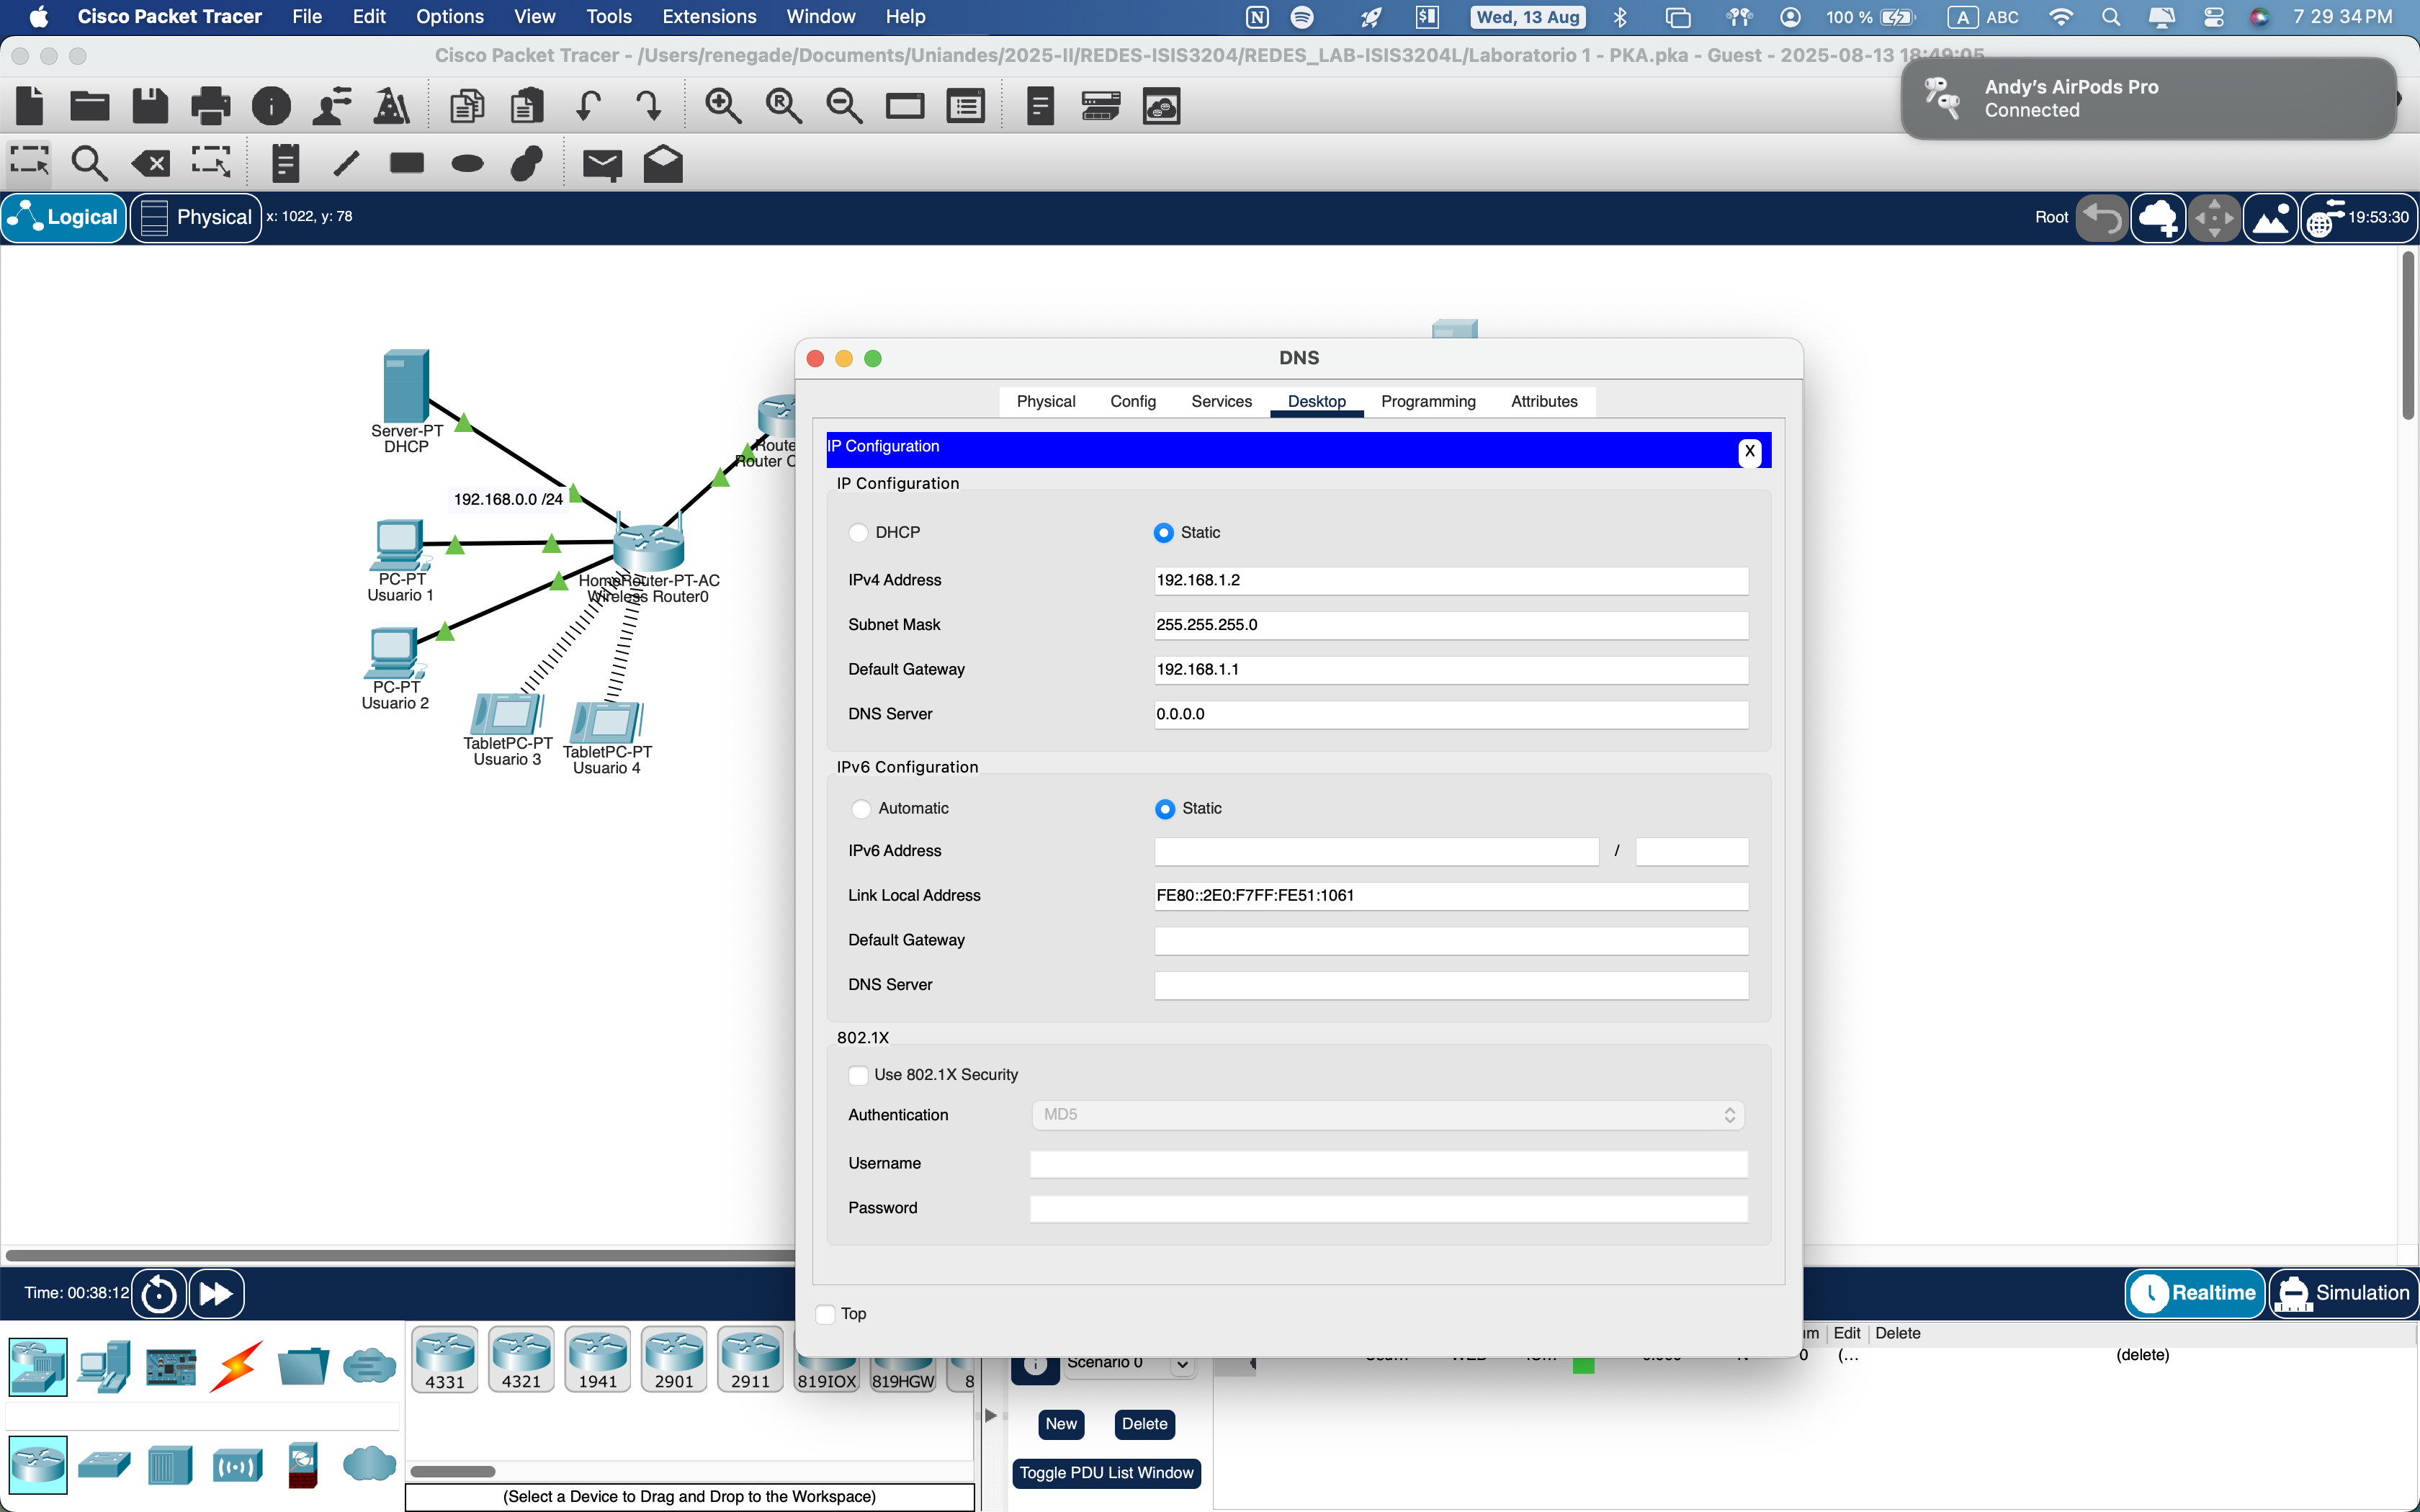
\includegraphics[width=0.65\textwidth]{lab-01-screenshots/41-1-DNS-ip-config.png}
    \caption{Ejemplo de configuración IP estática en el servidor DNS.}
\end{figure}

\subsection{Configuración del Servidor DHCP}

Para los clientes se habilitó un servidor DHCP en el Server5. De esta manera, los equipos de usuario obtienen su configuración automáticamente, lo cual simplifica la administración de la red.

El pool configurado contenía los siguientes parámetros:

\begin{itemize}
    \item \textbf{Default Gateway:} 192.168.0.1
    \item \textbf{DNS Server:} 192.168.1.2
    \item \textbf{Rango de direcciones:} 192.168.0.100 -- 192.168.0.255
    \item \textbf{Máscara de subred:} 255.255.255.0
    \item \textbf{Máximo número de usuarios:} 150
\end{itemize}

\begin{figure}[H]
    \centering
    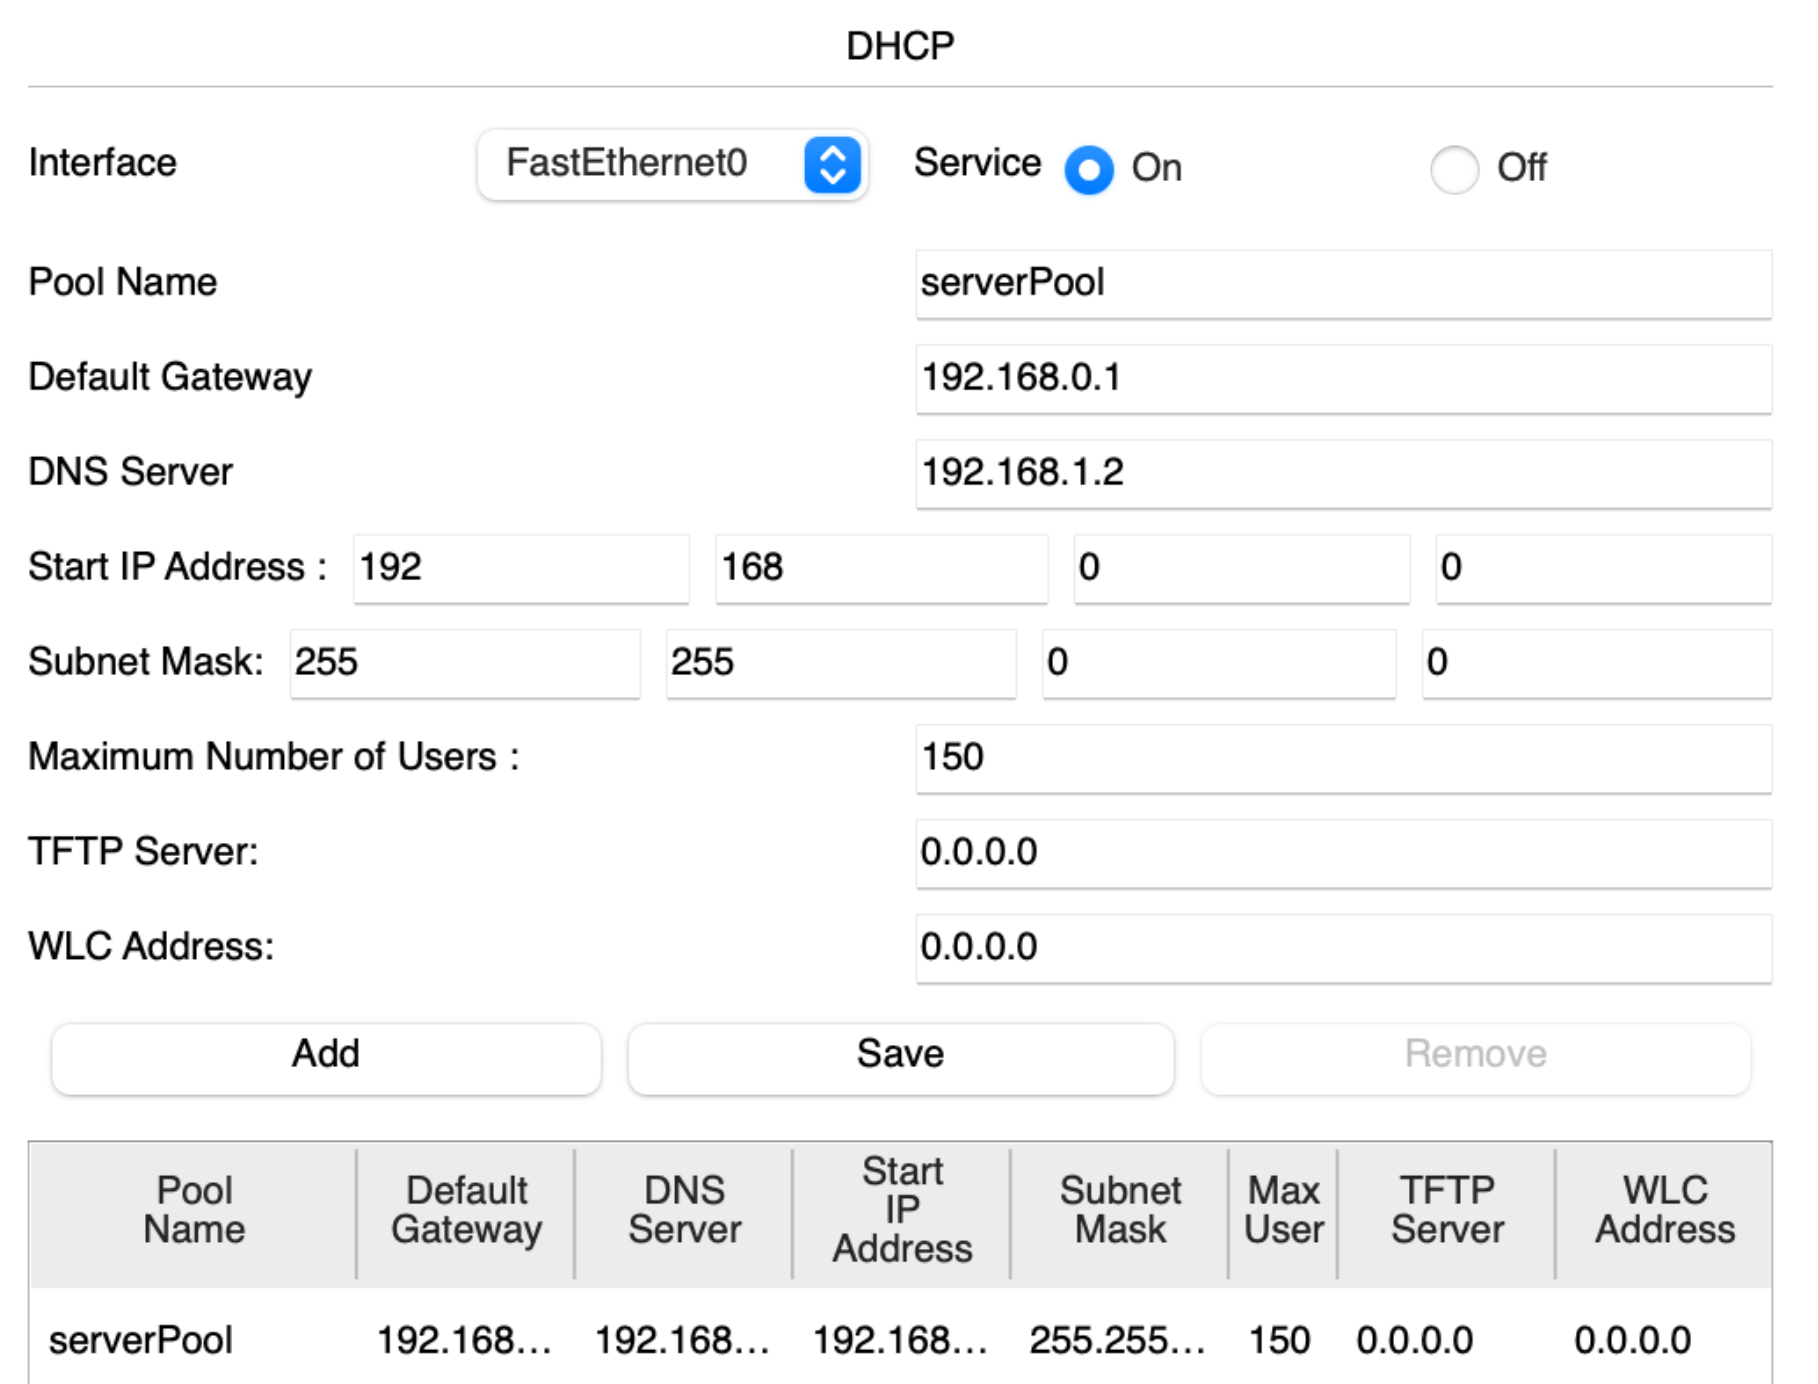
\includegraphics[width=0.65\textwidth]{lab-01-screenshots/41-5-DHCP-config.png}
    \caption{Configuración del servicio DHCP en el Server5.}
\end{figure}

\subsection{Asignación dinámica en clientes}

Cada usuario (PC1, PC2, PC3, PC4) fue configurado en modo DHCP. Al ejecutar seleccionar la opcion DHCP, se comprobó que los clientes recibieron direcciones dentro del rango definido, además del gateway y del servidor DNS.

\begin{figure}[H]
    \centering
    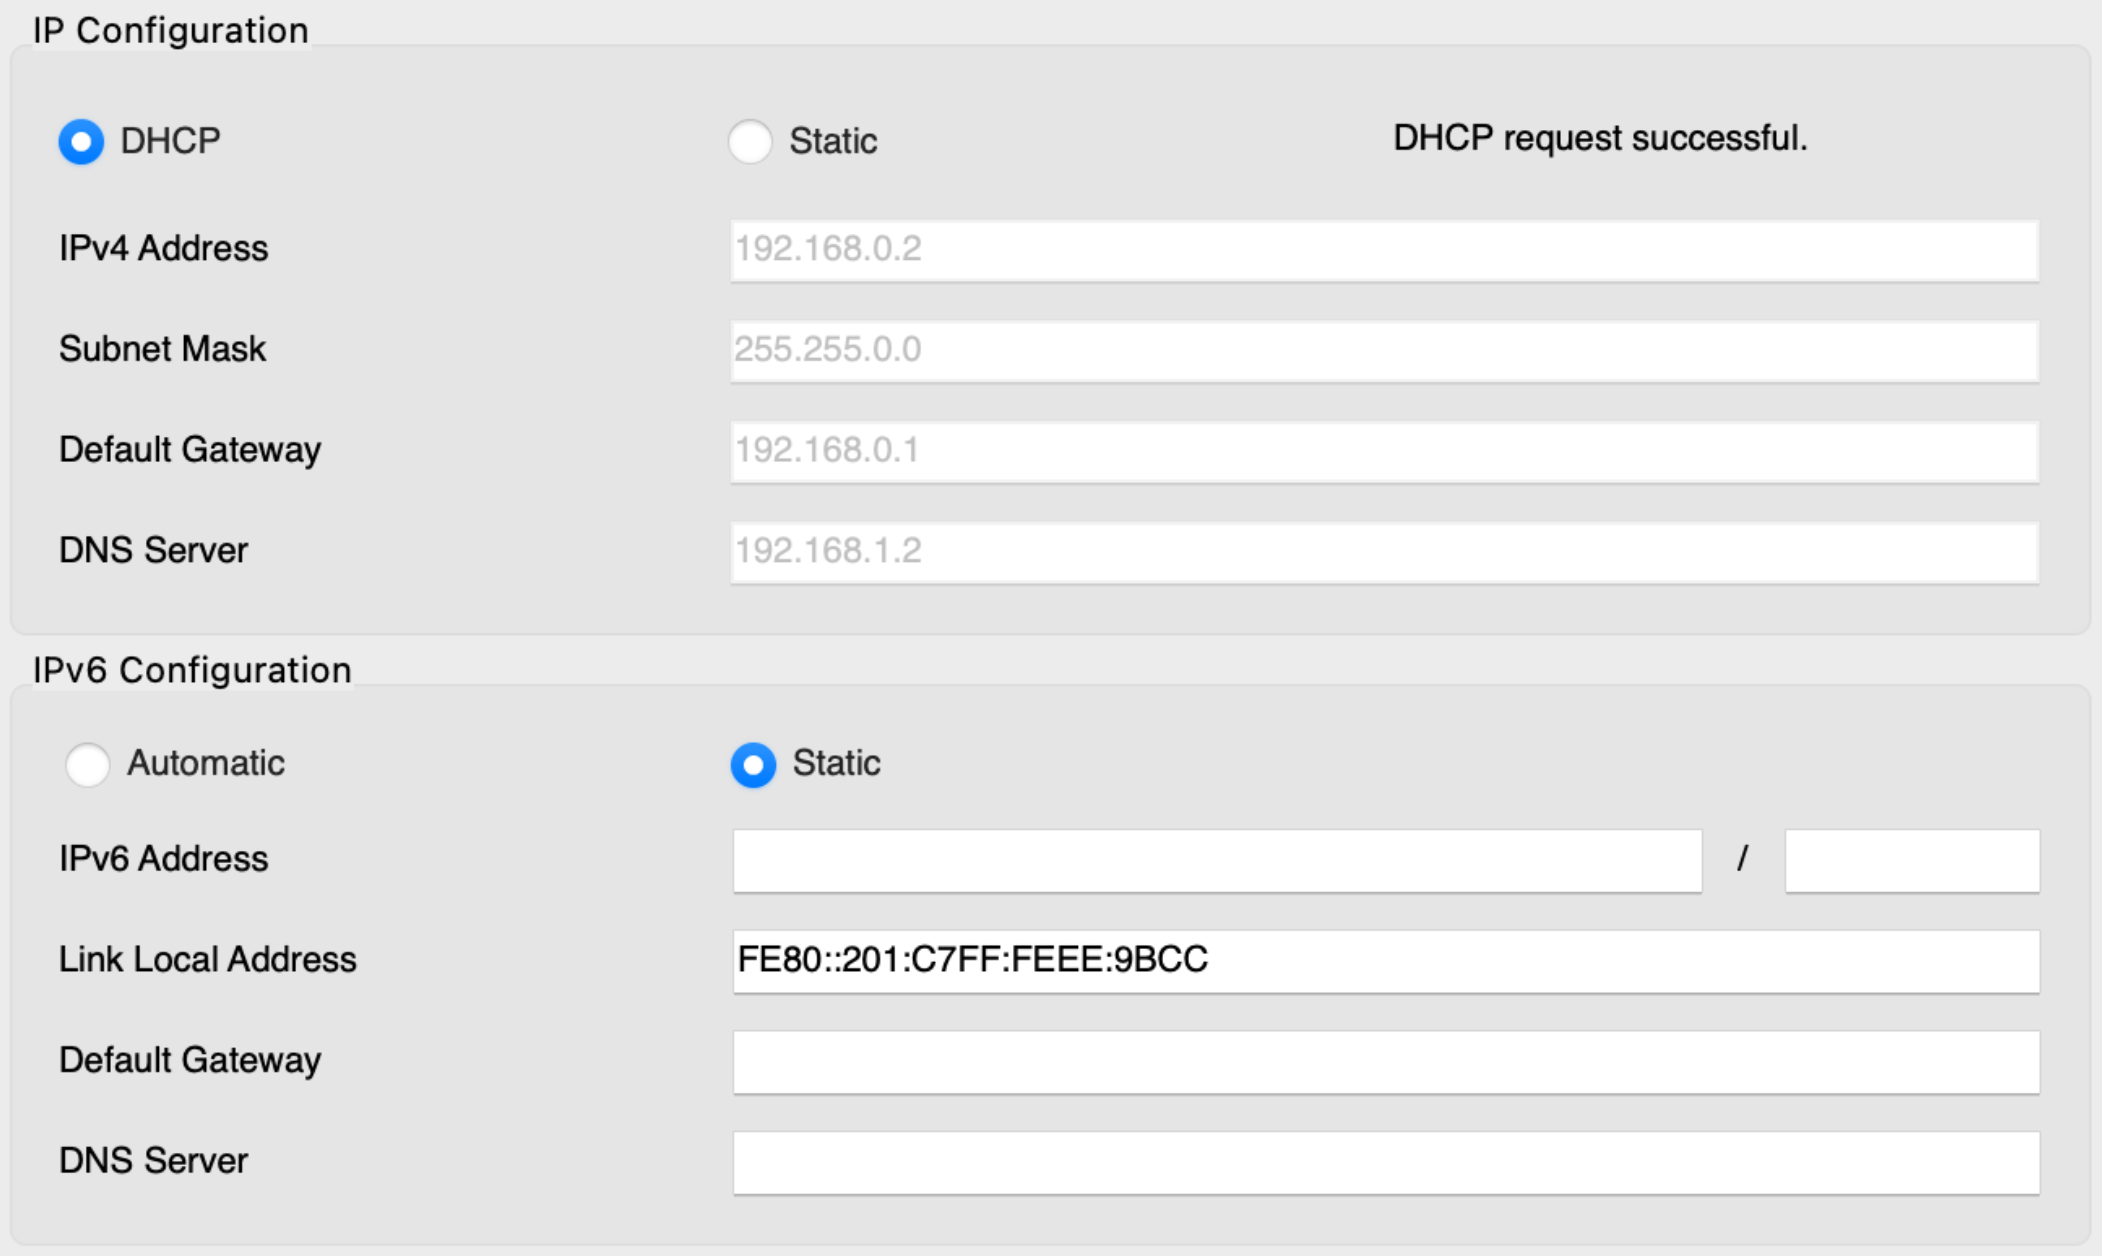
\includegraphics[width=0.65\textwidth]{lab-01-screenshots/41-6-user1-ip.png}
    \caption{Dirección IP obtenida dinámicamente por Usuario 1.}
\end{figure}

\bigskip
En conclusión, la red quedó con un direccionamiento mixto: los servidores con IP fija para garantizar disponibilidad, y los clientes con IP dinámica para mayor flexibilidad.

%==============================================================
%=====================   4.2   ================================
%==============================================================

\section{Configuración de servicio DNS}

El servicio DNS fue implementado en el Server1. Su propósito es \textbf{traducir nombres de dominio a direcciones IP}, de manera que los usuarios no tengan que recordar números, sino que puedan acceder a los servicios escribiendo su URL.

\subsection{Pasos realizados}

\begin{enumerate}
    \item Se deshabilitaron todos los servicios del servidor excepto el de \textbf{DNS}.
    \item En la pestaña de configuración de DNS, se agregaron registros de tipo \textbf{A Record}, asociando los nombres de dominio de los servicios con sus respectivas direcciones IP.
\end{enumerate}

\subsection{Registros configurados}

\begin{itemize}
    \item \texttt{dns.labredes.com} $\rightarrow$ 192.168.1.2
    \item \texttt{ftp.labredes.com} $\rightarrow$ 192.168.1.33
    \item \texttt{mail.labredes.com} $\rightarrow$ 192.168.1.34
    \item \texttt{web.labredes.com} $\rightarrow$ 192.168.1.35
\end{itemize}

\begin{figure}[H]
    \centering
    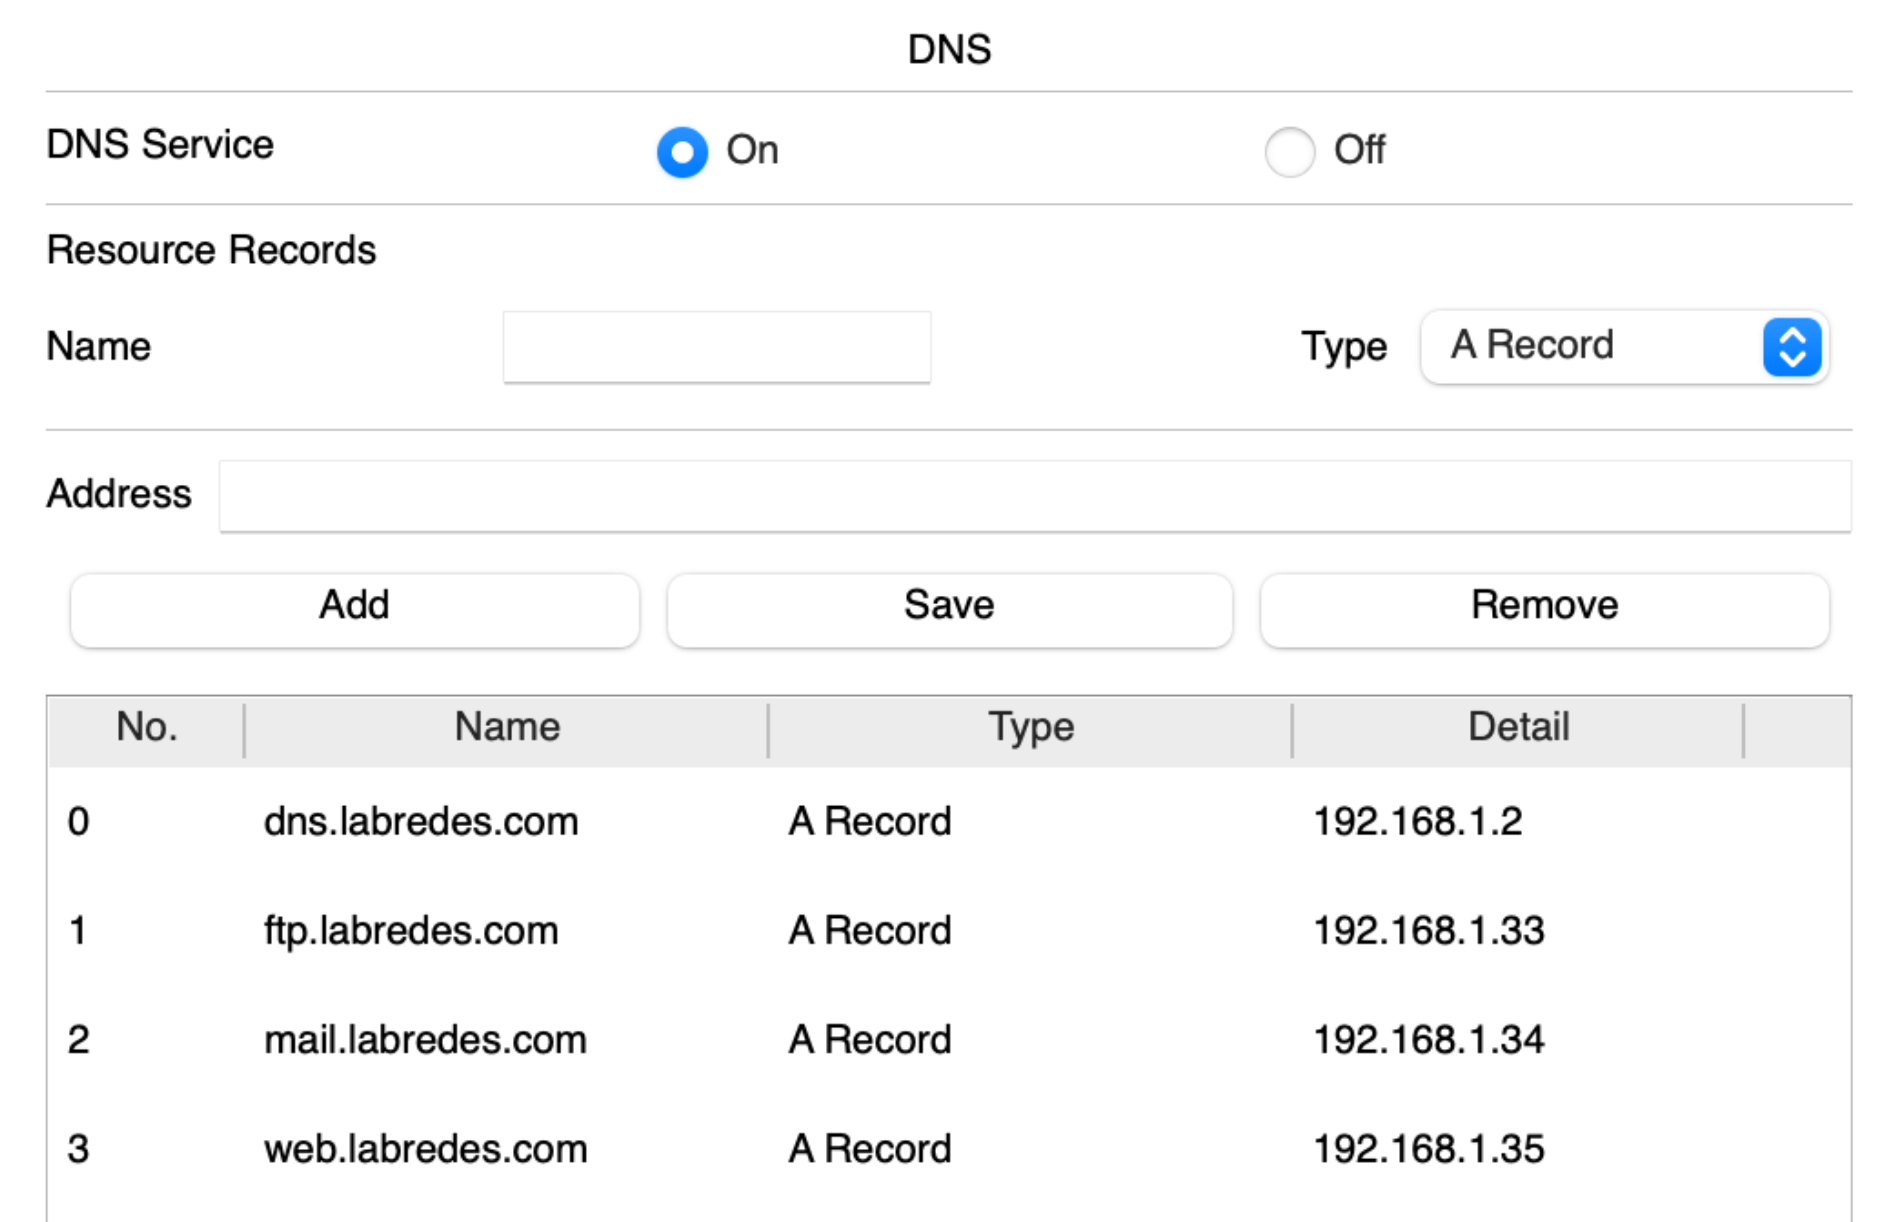
\includegraphics[width=0.65\textwidth]{lab-01-screenshots/42-1-DNS-config.png}
    \caption{Registros DNS configurados en el servidor.}
\end{figure}

\bigskip
Gracias a esta configuración, al realizar pruebas desde los clientes se logró acceder a los servicios tanto por dirección IP como por nombre de dominio. Esto demuestra el correcto funcionamiento del servidor DNS dentro de la red diseñada.

%==============================================================
%=====================   4.3   ================================
%==============================================================
\section{Pruebas de Conectividad (Comando ping) y Exploración del Protocolo DNS}

Para este punto vamos a probar la correcta conectividad de los equipos de los clientes y, sobretodo, verificaremos el correcto funcionamiento del servidor DNS, esto a traves del comando \textbf{ping} mostrandonos el tiempo de respuesta del servidor y si es accesible o no.

\subsection{Obtener direcciones ip usuarios}
Se hallaron las ip de los 4 usuarios, haciendo uso del comando \textbf {ipconfig}, asi como lo muestra la figura 5, la cual muestra la ejecución de este comando para el usuario 1.
\begin{figure}[H]
    \centering
    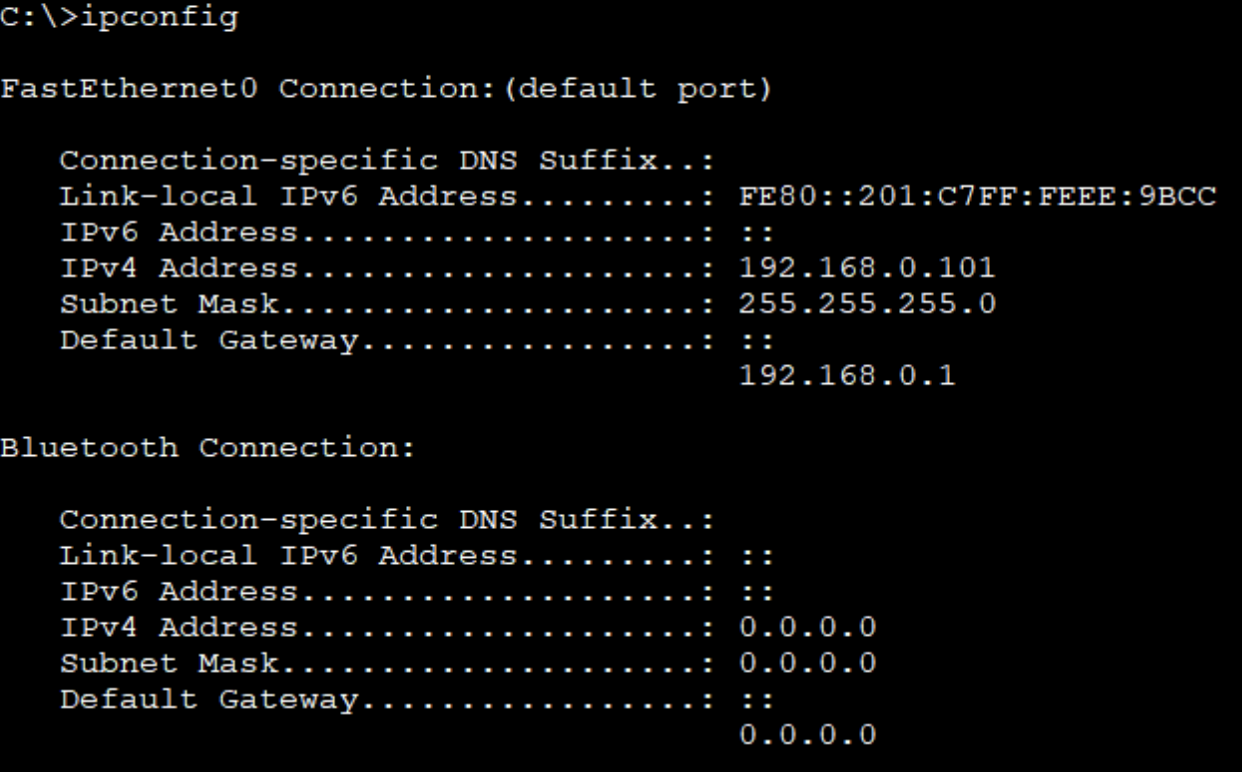
\includegraphics[width=0.65\textwidth]{lab-01-screenshots/43 ipconfig.png}
    \caption{Ejecucion ipconfig en la maquina de usuario 1.}
\end{figure}
 Tambien adjuntamos las ip halladas usando el comando de \textbf{ipconfig} para los 4 usuarios
\begin{itemize}
    \item \texttt{Usuario 1} $\rightarrow$ 192.168.0.101
    \item \texttt{Usuario 2} $\rightarrow$ 192.168.0.100
    \item \texttt{Usuario 3} $\rightarrow$ 192.168.0.102
    \item \texttt{Usuario 4} $\rightarrow$ 192.168.0.103
\end{itemize}
\subsection{Prueba ping a los diferentes usuarios}
A continuacion haremos uso del comando ping desde el usuario 1 hacia los demas usuarios para verficar la correcta conexion de todos los usuarios a la red. Esto usuando el comando \textbf {ping} como se muestra a continuación.
\begin{figure}[H]
    \centering
    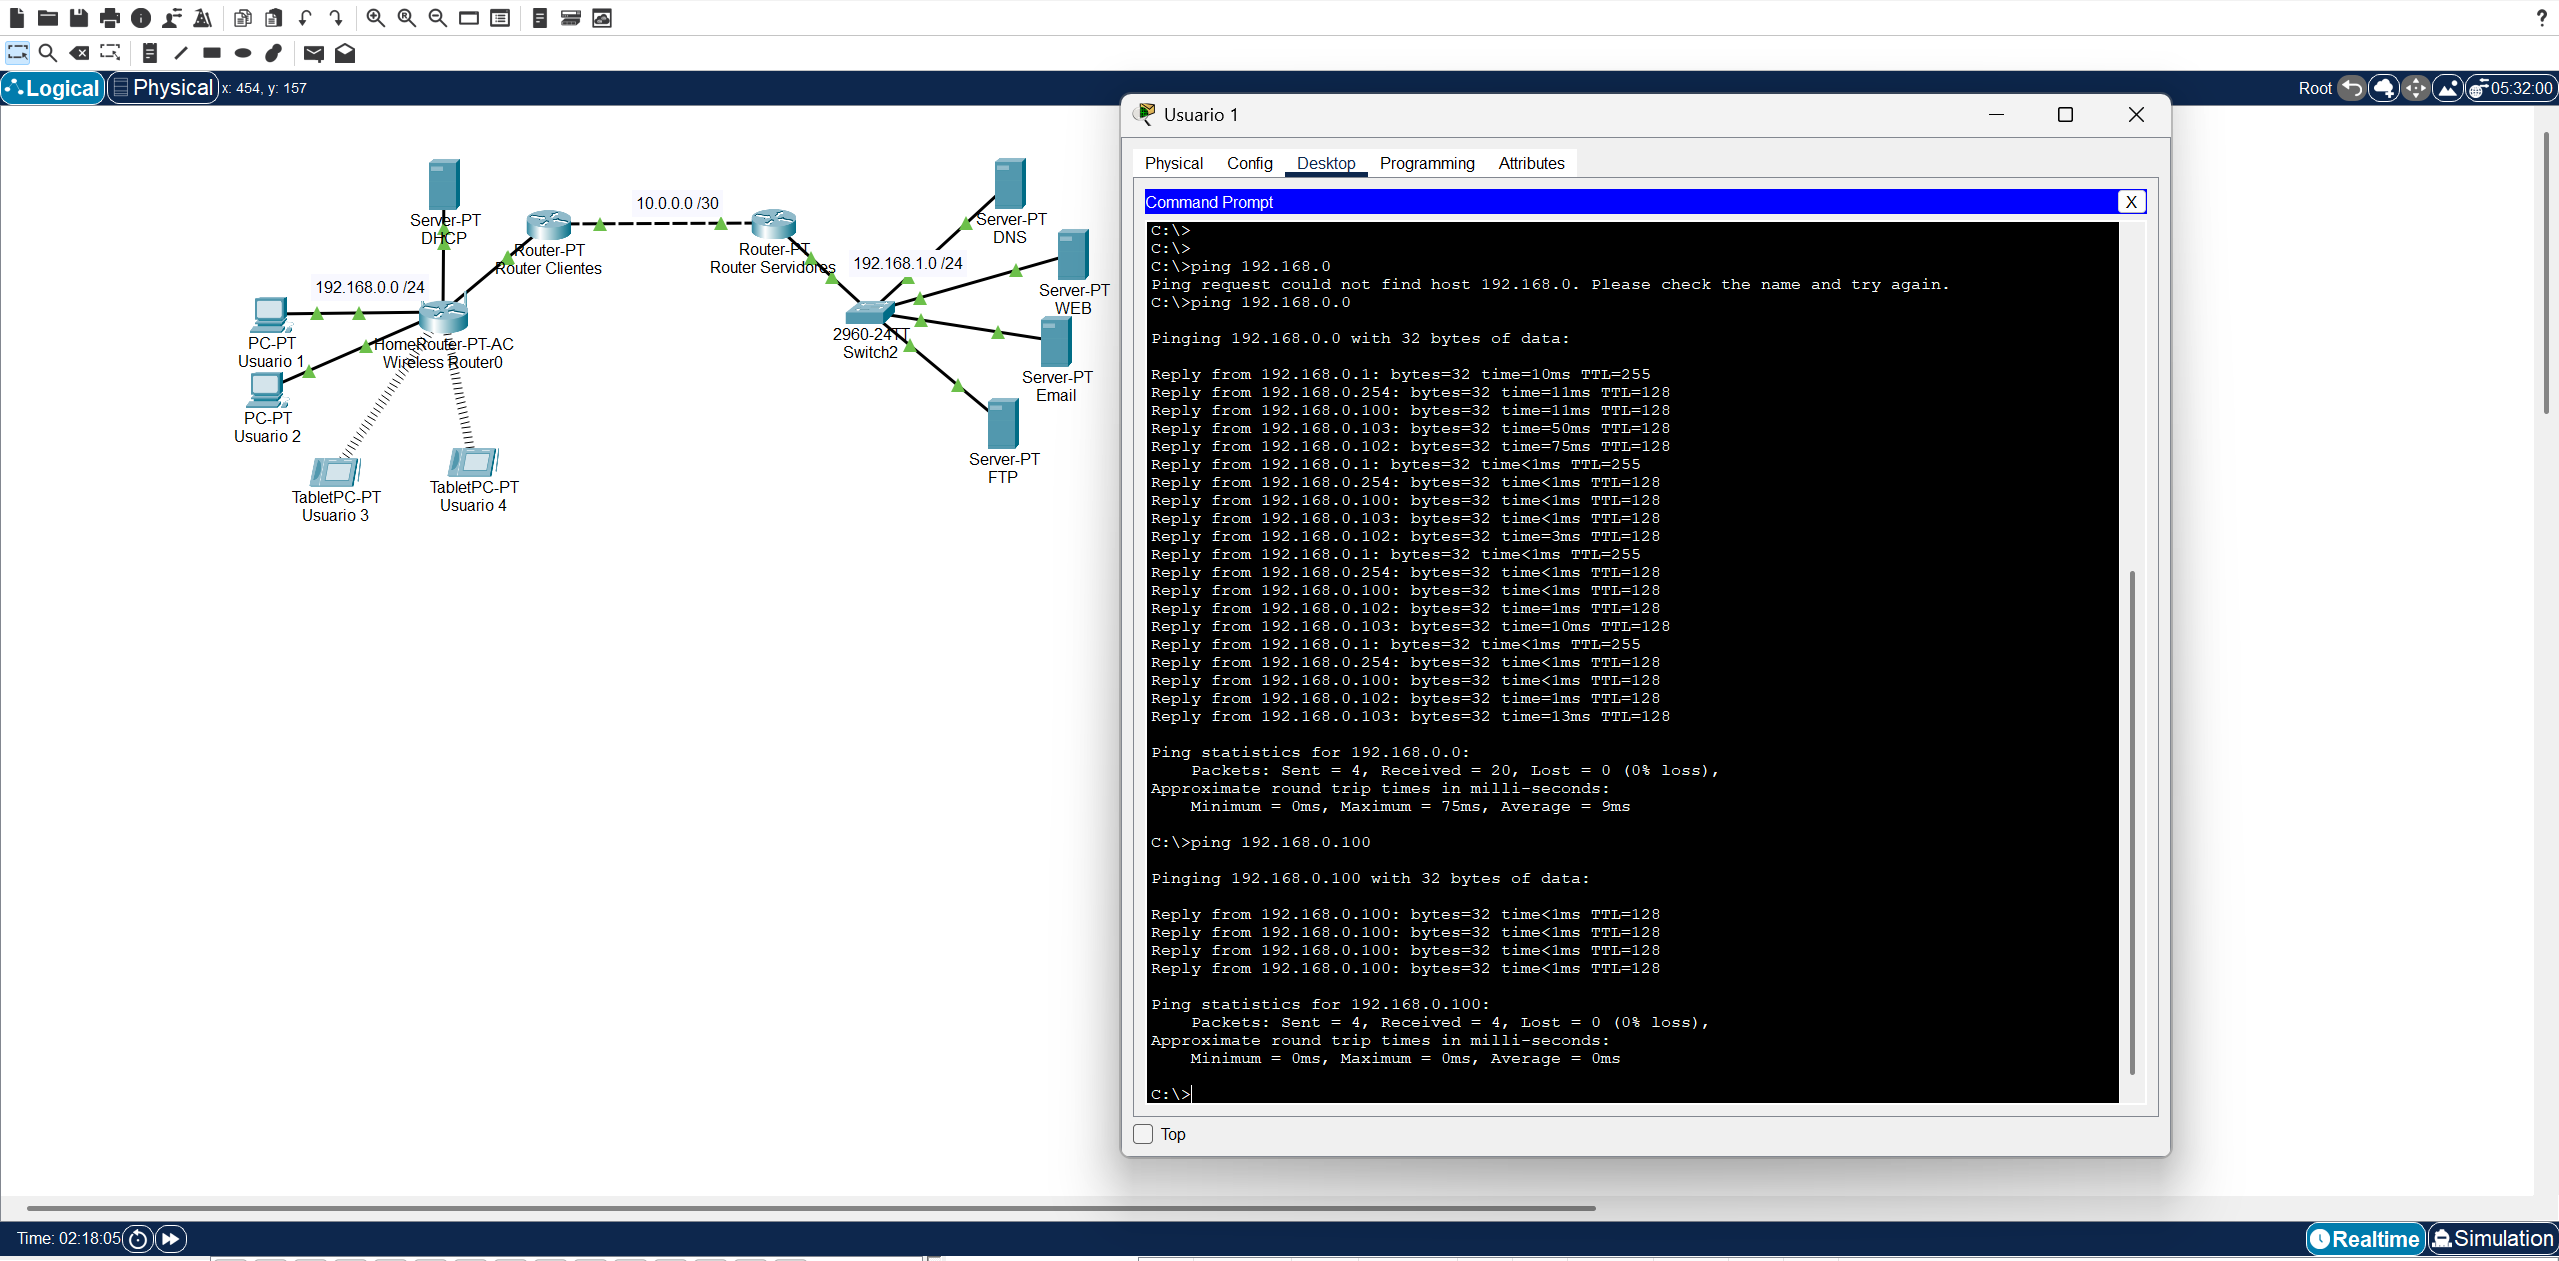
\includegraphics[width=0.65\textwidth]{lab-01-screenshots/43 -2-ping-local.png}
    \caption{Ping desde usuario 1 a los demas dispositivos conectados en la parte de la red de clientes.}
\end{figure}
Como se ve en la figura 6, usando el comando \textbf {ping}, no solo encontramos que los otros 3 usuarios estan en linea, sino tambien pudimos encontrar que el servidor DHCP tambien nos devlvio una respuesta, al igual que el "Router Clientes".

\subsection{Ping al servidor web}
Seguiremos con un ping al servidor web, el cual cuenta con la dirección ip estatica 192.168.1.35. Como podremos observar en la figura 6 contaremos con una respuesta positiva por parte del servidor.
\begin{figure}[H]
    \centering
    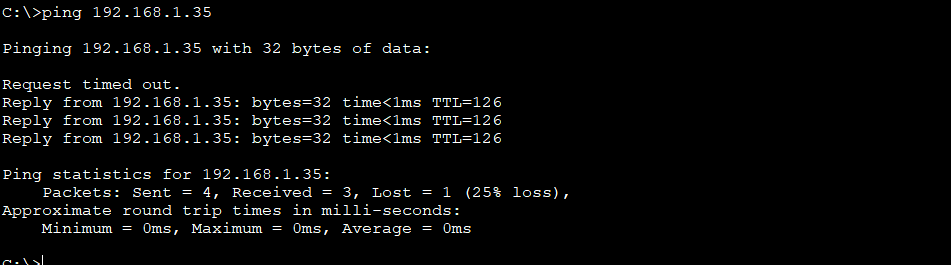
\includegraphics[width=0.65\textwidth]{lab-01-screenshots/43-2-ping-web.png}
    \caption{Ping desde usuario 1 al servidor web.}
\end{figure}
En la figura 7 tambien podemos observar que el primer paquete de bytes se pierde, esto se da porque para el primer paquete no se ha enrutado con el MAC del servidor y no se logra dar una respuesta a tiempo, cosa que no sucede para el resto de los paquetes.
\subsection{Ping web.labredes.com}
Vamos entonces a hacer una prueba de conectividad al servidor web y al mismo tiempo, una prueba del correcto funcionamiento del servidor dns, el cual permite que al hacer ping a \textit {web.labredes.com} y que este se conecte a la ip de nuestro servidor. 
\begin{figure}[H]
    \centering
    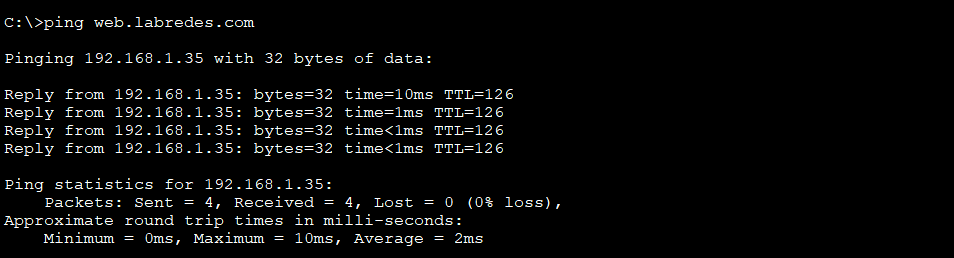
\includegraphics[width=0.65\textwidth]{lab-01-screenshots/43-3-ping-web.png}
    \caption{Ping desde usuario 1 al servidor web usando su url.}
\end{figure}
Como vemos en la figura 8, tenemos que la respuesta del ping es favorable, y ademas, responde desde la IP estatica que configuramos para nuestro servidor web, demostrando asi que el servidor \textbf {DNS} quedo correctamente configurado.
\subsection{Ejecutar nslookup}
\textbf{nslookup} es un comando que nos dice la direccion IP asociada a cierto dominio, el servidor donde esta alojado y la direccion IP del mismo. 
\begin{figure}[H]
    \centering
    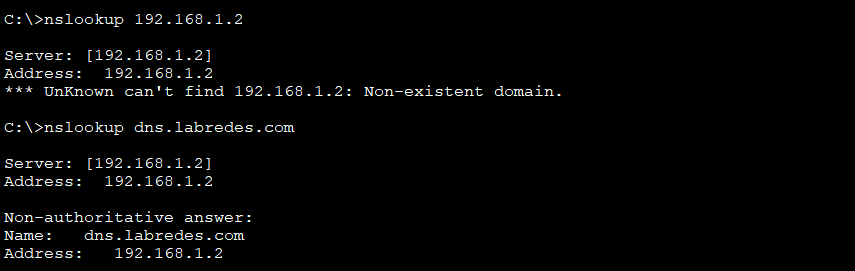
\includegraphics[width=0.65\textwidth]{lab-01-screenshots/43-4-nslookup.png}
    \caption{Ejecucion del comando nslookup.}
\end{figure}
Como vemos en la figura 9 el comando \textbf{nslookup} no solo nos dice la informacion de un servidor, sino que tambien nos puede decir si cierto dominio es inexistente. Util para hallar informacion a cerca de los servidores asociados a un dominio o para solucionar problemas que puedan estar relacionados al DNS.

%==============================================================
%=====================   4.4   ================================
%==============================================================
\section{Configuración y Exploración del servidor WEB}
Para esta punto del laboratorio buscaremos configurar el servidor web, con los protocolos \textit{HTTP y HTTPS} Teniendo en cuenta que, como vimos en los puntos anteriores, ya hemos configurado el DNS y su IP para asegurar su correcto funcionamiento.
\subsection{Habilitar servicios HTTP y HTTPS}
\begin{figure}[H]
    \centering
    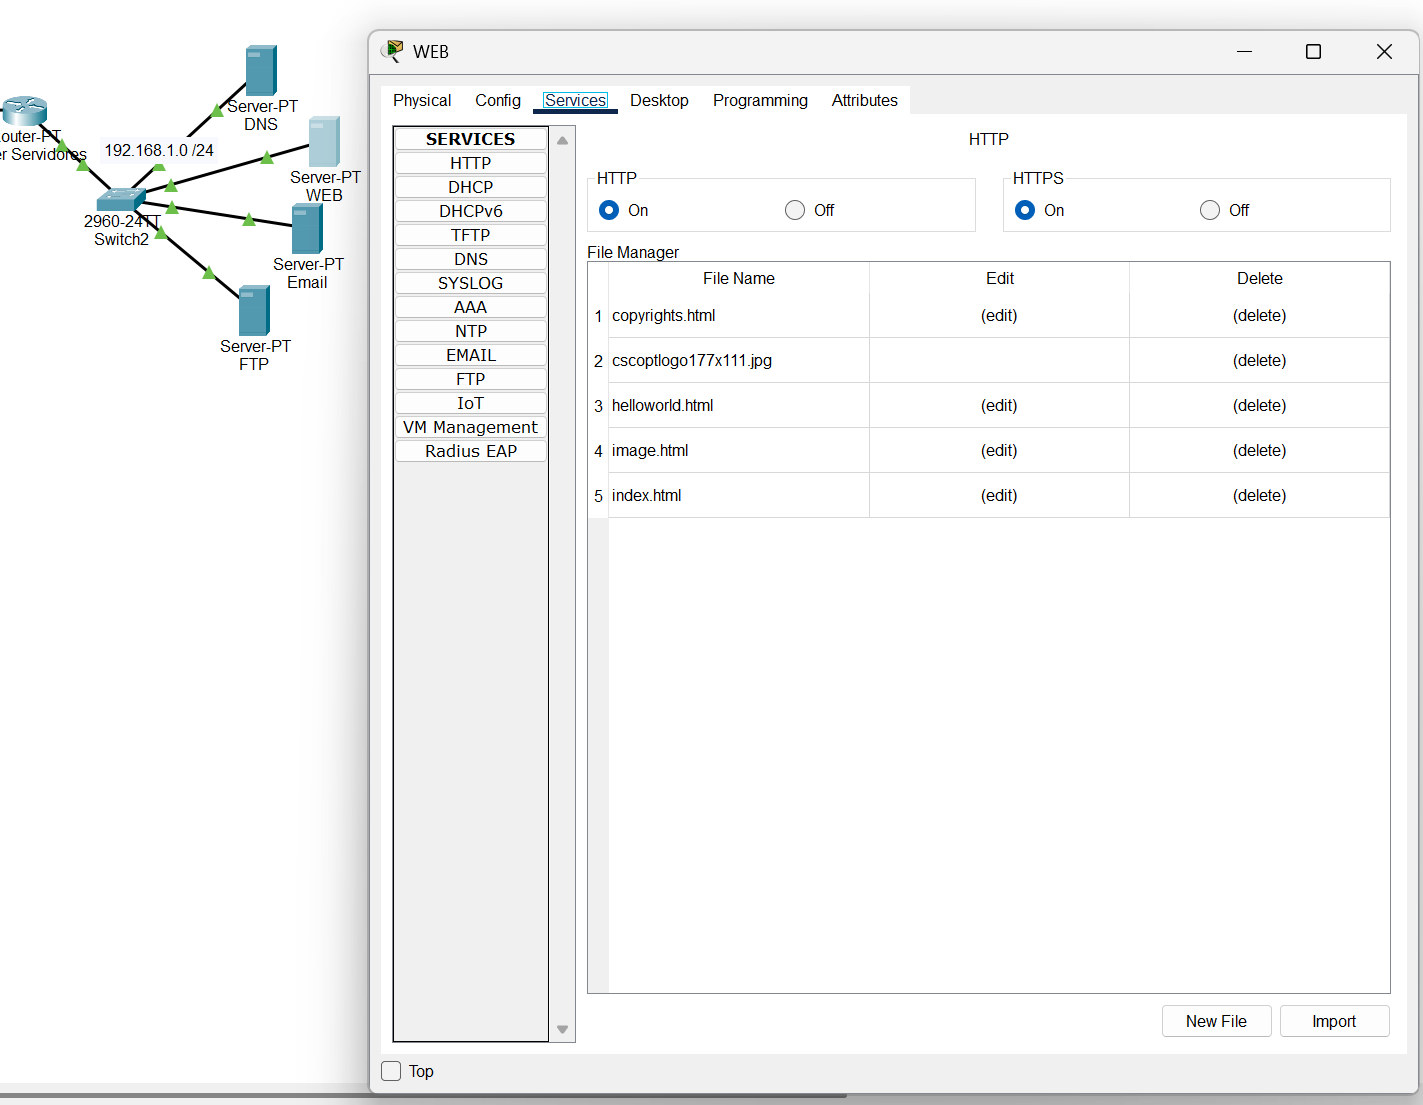
\includegraphics[width=0.65\textwidth]{lab-01-screenshots/44-1-config-server.png}
    \caption{Ejecucion del comando nslookup.}
\end{figure}
En la figura 10 podemos ver como activamos los servicios de web (\textit{HTTP y HTTPS}) para poder acceder por medio de las tecnologias web, como un buscador, a las diferentes paginas que se tengan cargadas en el servidor.
\subsection{Creacion de paginas de presentacion}
\begin{figure}[H]
    \centering
    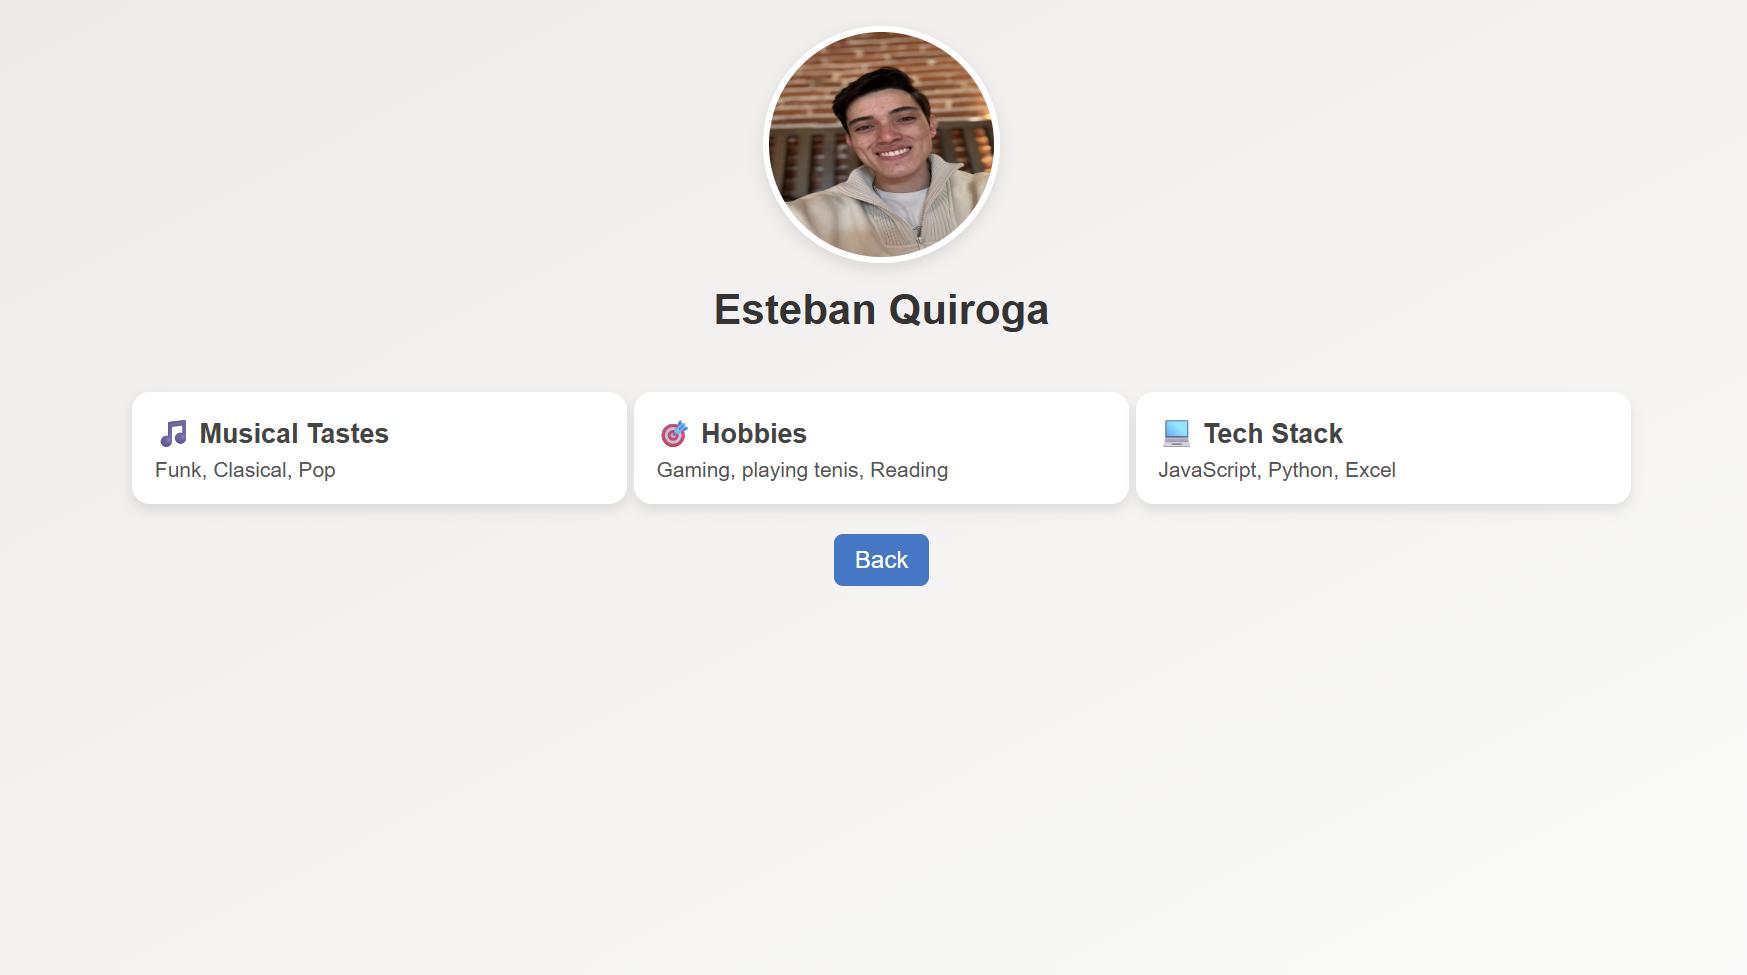
\includegraphics[width=0.65\textwidth]{lab-01-screenshots/44-1-presentacion.png}
    \caption{Pagina de presentacion Esteban Quiroga.}
\end{figure}
En la figura 11 vemos la pagina de presentacion para el compañero Esteban Quiroga, donde se ven sus intereses, gustos musicales, entre otros.
\subsection{Pruebas de conectividad servicios HTTP y HTTPS}
\begin{figure}[H]
    \centering
    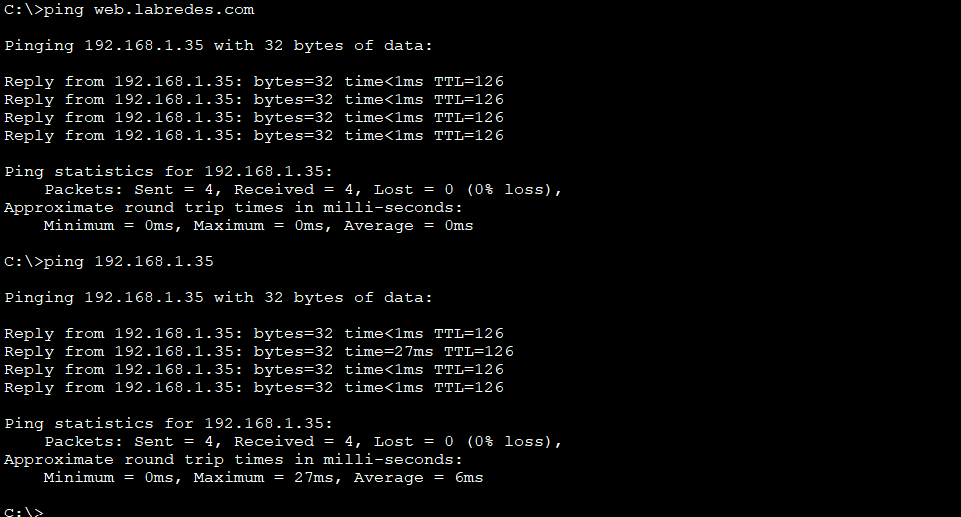
\includegraphics[width=0.65\textwidth]{lab-01-screenshots/44-2-prueba.png}
    \caption{Prueba de conexion servidor web.}
\end{figure}
En la figura 12 podemos ver la respuesta positiva usando el comando \textit{ping} para el servidor, tanto usando su IP, como usando su correspondiente URL.
\subsection{Prueba de conexion HTTP usando el buscador}
\begin{figure}[H]
    \centering
    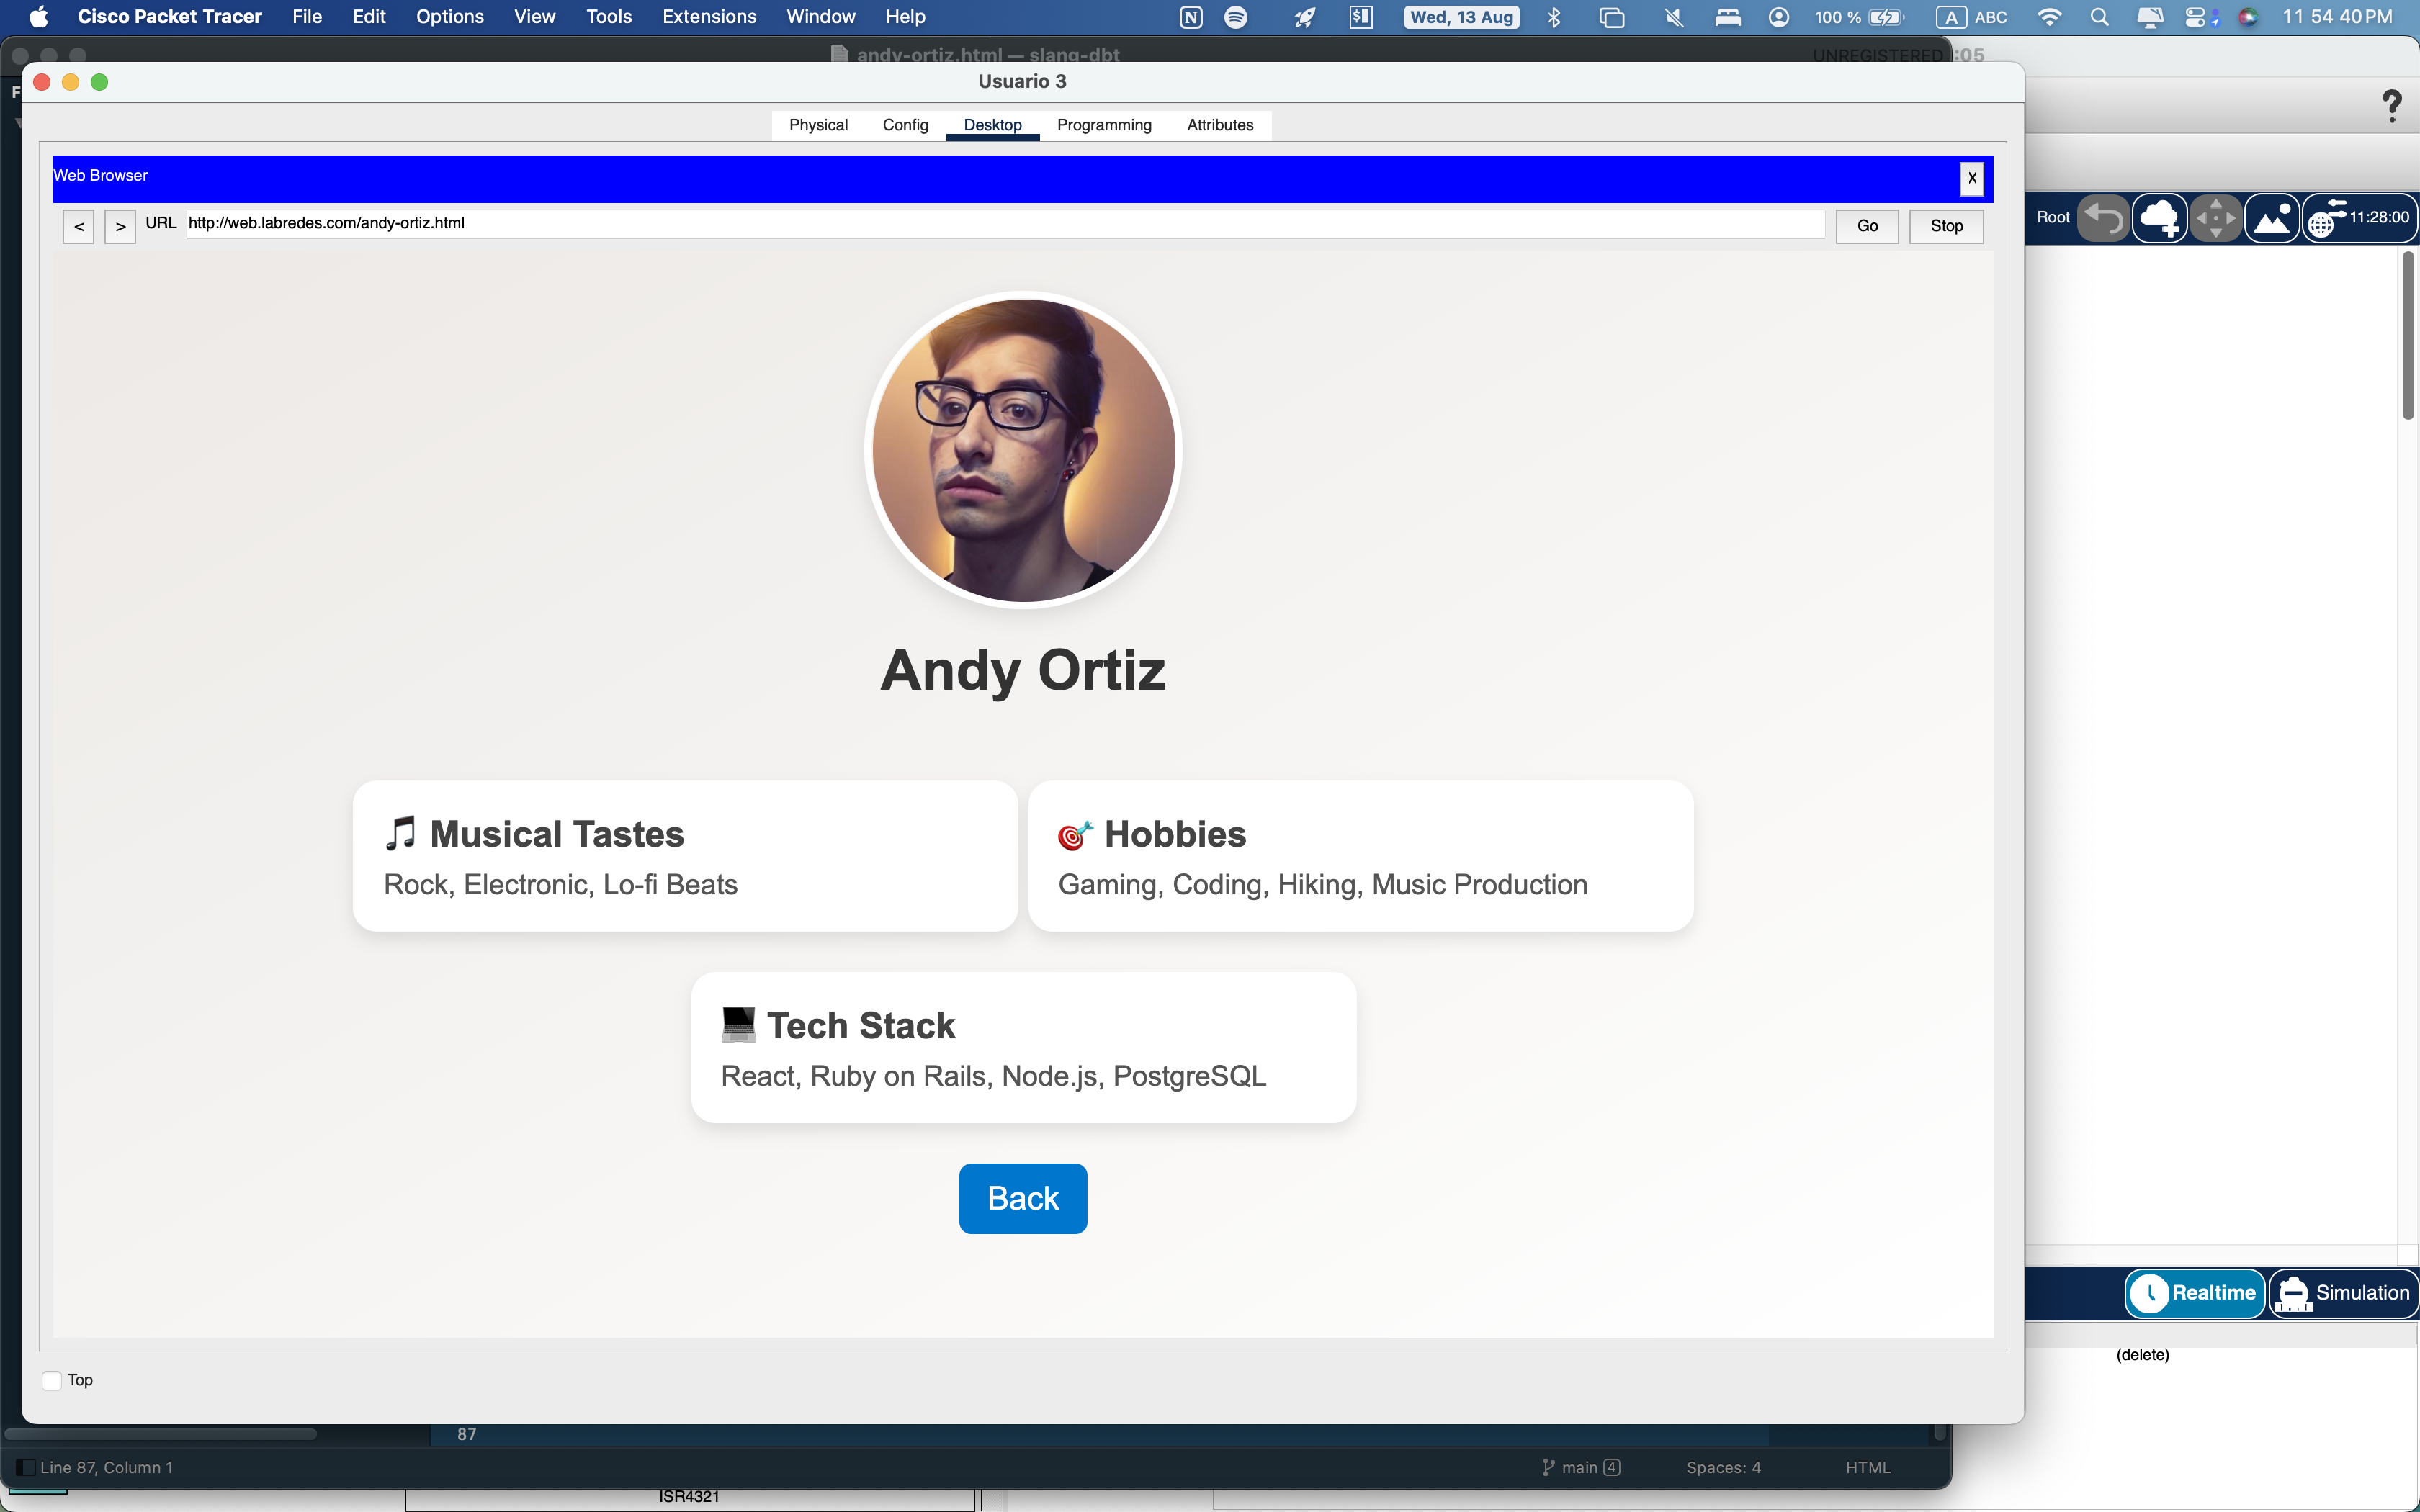
\includegraphics[width=0.65\textwidth]{lab-01-screenshots/44-2-andy-profile.png}
    \caption{Prueba de conexion exitosa usando HTTP.}
\end{figure}
En la figura 13 podemos ver como la conexion al servidor web fue exitosa usando el protocolo web HTTP, pues la pagina de perfil de Andy cargo correctamente usando este protocolo.
\subsection{Prueba de conexion HTTP usando el buscador}
\begin{figure}[H]
    \centering
    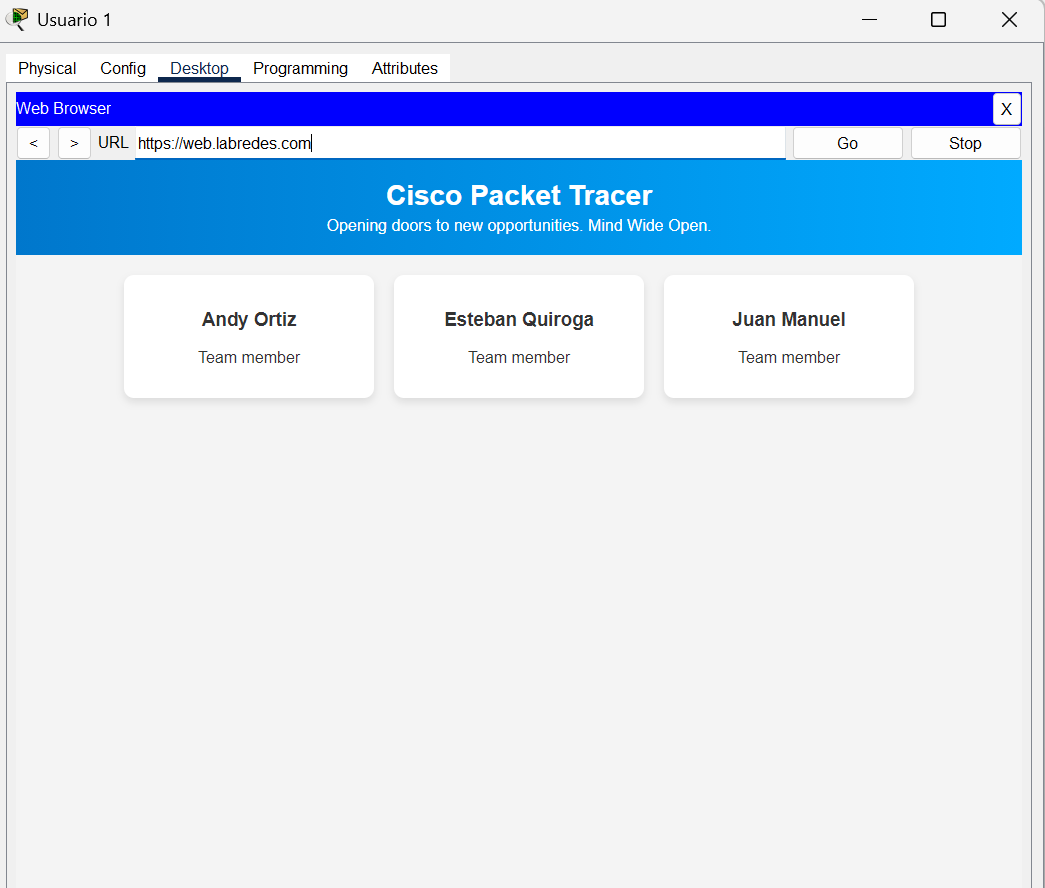
\includegraphics[width=0.65\textwidth]{lab-01-screenshots/44-3-https.png}
    \caption{Prueba de conexion exitosa usando HTTPS.}
\end{figure}
En la figura 14 podemos ver como la conexion al servidor web fue exitosa usando el protocolo web HTTPS, pues la pagina \textit{index} cargo exitosamente, demostrando asi con el paso anterior que ambos servicios estan en linea y funcionando segun lo esperado.

%==============================================================
%===========================  4.5   ===========================
%==============================================================
\section{Configuración y exploración de los protocolos de correo electrónico SMTP y POP3}
En esta sección del laboratorio, realizamos la configuración y validación de servicios de email en la red simulada. Para lograrlo, activamos SMTP y POP3 en el servidor de email (192.168.1.34) para enviar emails de un cliente a otro y recuperar los emails en el cliente destino.
\subsection{Configuración de email server}
Configuramos el servidor de email para que no ofrezca servicios que no tengan que ver con email. Habilitamos el servicio SMTP que escucha en el puerto 25 y funciona para que los clientes puedan enviar emails. También habilitamos el servicio POP3 que escucha en el puerto 110 y funciona para que los clientes puedan recibir emails. Juntos, estos protocolos completan el ciclo de comunicación por email. Adicionalmente, se agregaron usuarios y contraseñas para cada miembro del grupo. Estas credenciales sirven para autenticar a cada cliente al enviar (SMTP) y recibir (POP3) mensajes, asegurando que cada usuario solamente tenga acceso a su propio mailbox.


\begin{figure}[H]
    \centering
    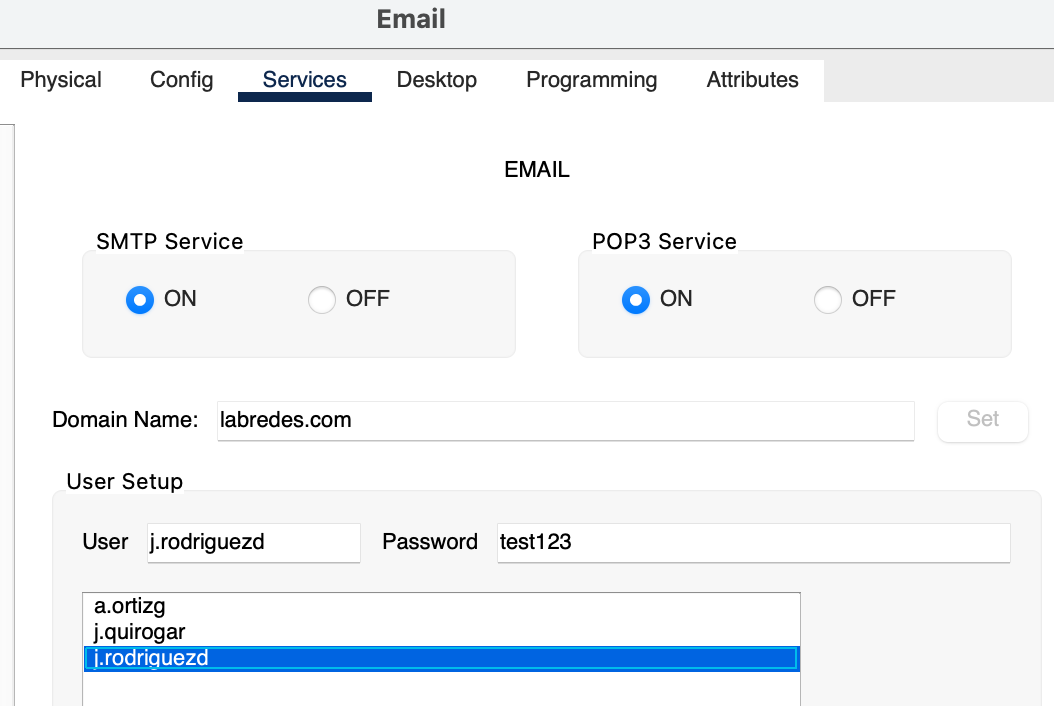
\includegraphics[width=0.65\textwidth]{lab-01-screenshots/45-1-email-config.png}
    \caption{Configuracion de email server}
\end{figure}


\subsection{Prueba de conectividad al email server}
En este paso se realizó una prueba de conectividad para asegurar que el servidor de email sea alcanzable desde las máquinas de los clientes. Si el cliente que realiza el \textbf{ping} obtiene respuestas, significa que el enrutamiento entre la subred del usuario y la subred del servidor de email está correcto.

\begin{figure}[H]
    \centering
    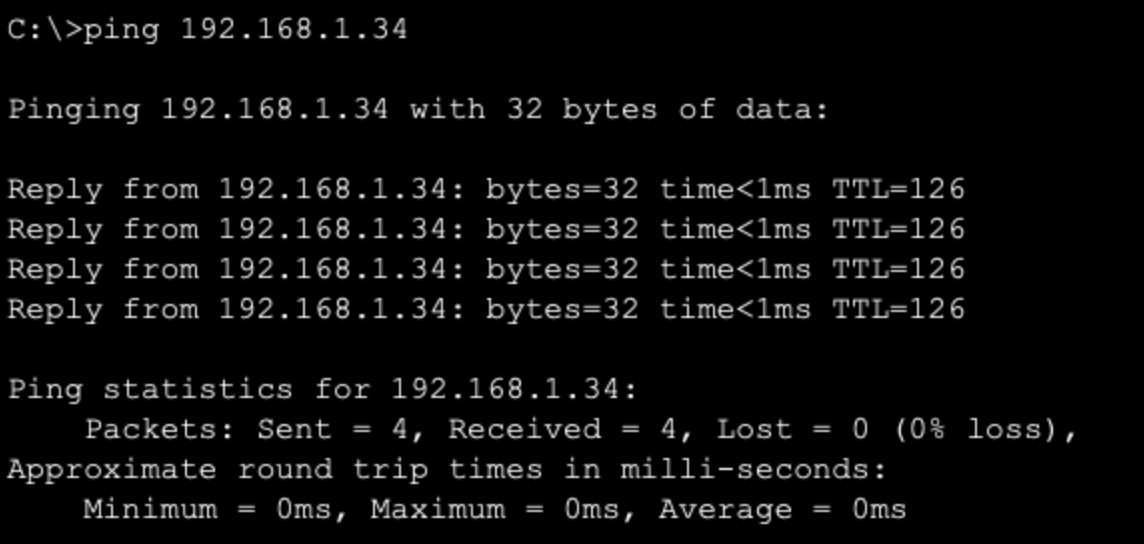
\includegraphics[width=0.65\textwidth]{lab-01-screenshots/45-2-ping-email}
    \caption{\textbf{ping} al email server}
\end{figure}

Esta prueba es importante ya que SMTP ni POP3 van a funcionar correctamente si falla el ping, ya que esos protocolos de la capa de aplicación dependen de que la conexión TCP esté funcionando.

\subsection{Configuración de emails en maquinas de cliente}

\begin{figure}[H]
    \centering
    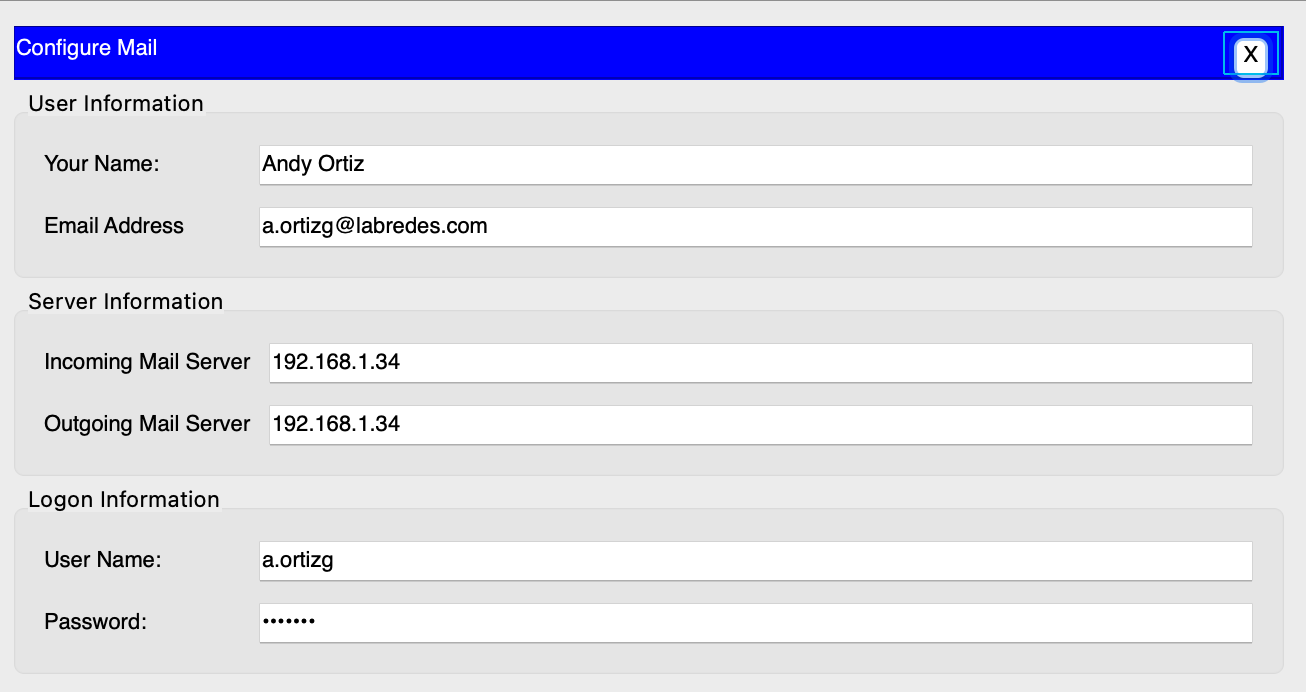
\includegraphics[width=0.65\textwidth]{lab-01-screenshots/45-3-client-config.png}
    \caption{Configuración cliente email para a.ortizg}
\end{figure}

Después de verificar que sea posible establecer una conexión entre los clientes y el servidor de email, configuramos a cada usuario en las máquinas de los clientes con su respectivo email, contraseña, y la información del servidor de email. Esta configuración le deja saber al servidor de email quién es el usuario y a dónde debe dirigir correos destinados a un usuario en particular.

\subsection{Envío y recepción de correos entre clientes}
Al realizar las configuraciones de los clientes, podemos enviar un mensaje de un cliente a otro. A continuacion describimos los pasos para realizar esta comunicacion:
\begin{enumerate}
\item \textit{a.ortizg} escribe un mensaje para \textit{j.quirogar}
\item Por medio de SMTP \textit{a.ortizg} manda el mensaje al email server
\item El email server lo recibe y lo mete en el buzón de \textit{j.quirogar}
\item Cuando el cliente de \textit{j.quirogar} revisa su buzón, se conecta con POP3, se autentica, y descarga el mensaje
\item El mensaje es mercado para eliminacioón del email server (si se elimina del cliente, desaparece para siempre)
\end{enumerate}


\begin{figure}[H]
    \centering
    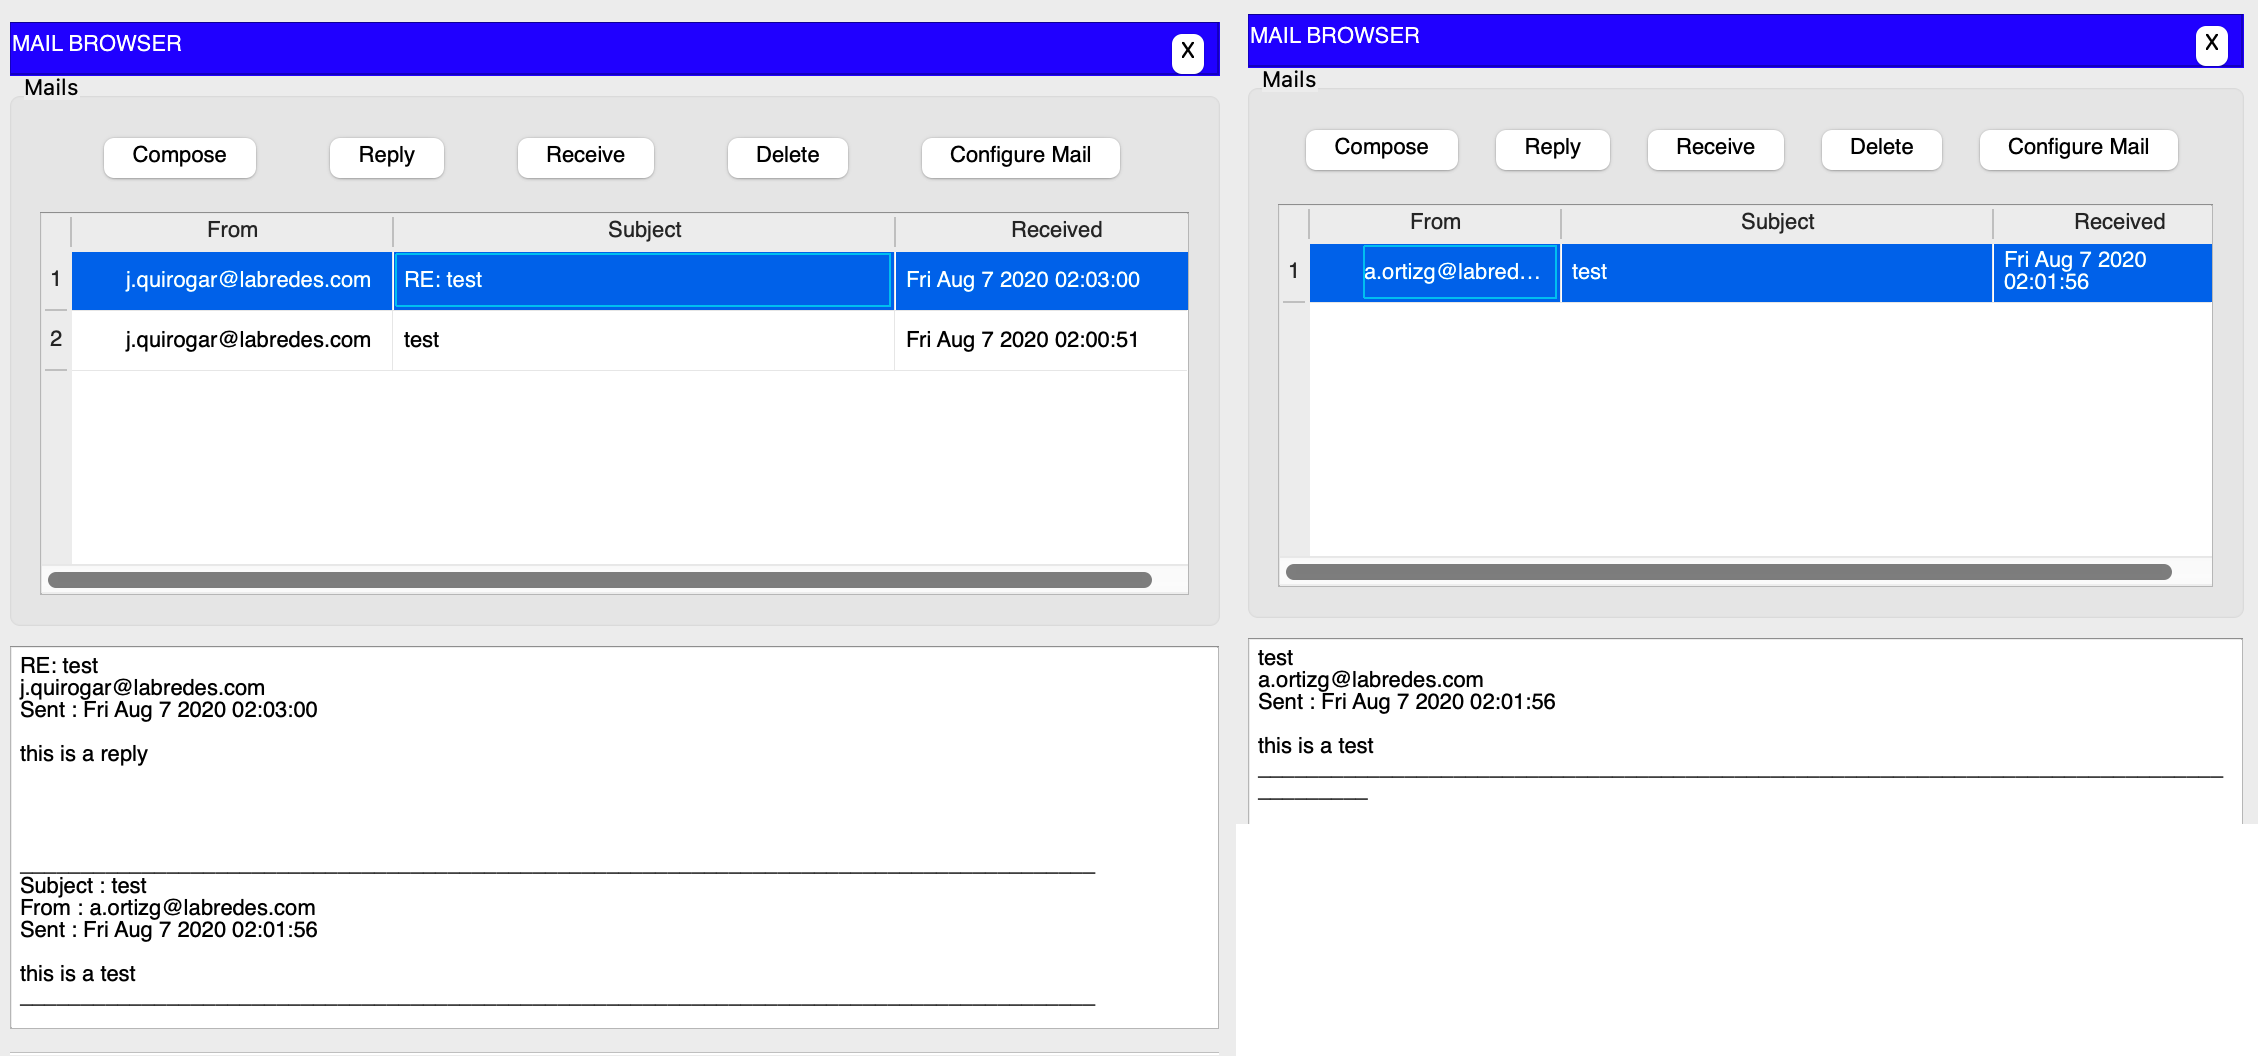
\includegraphics[width=0.65\textwidth]{lab-01-screenshots/45-4-send-receive.png}
    \caption{Enviando/recibiendo un email}
\end{figure}

%==============================================================
%===========================  4.6   ===========================
%==============================================================
\section{Configuración y exploración de protocolo FTP}

\begin{figure}[H]
    \centering
    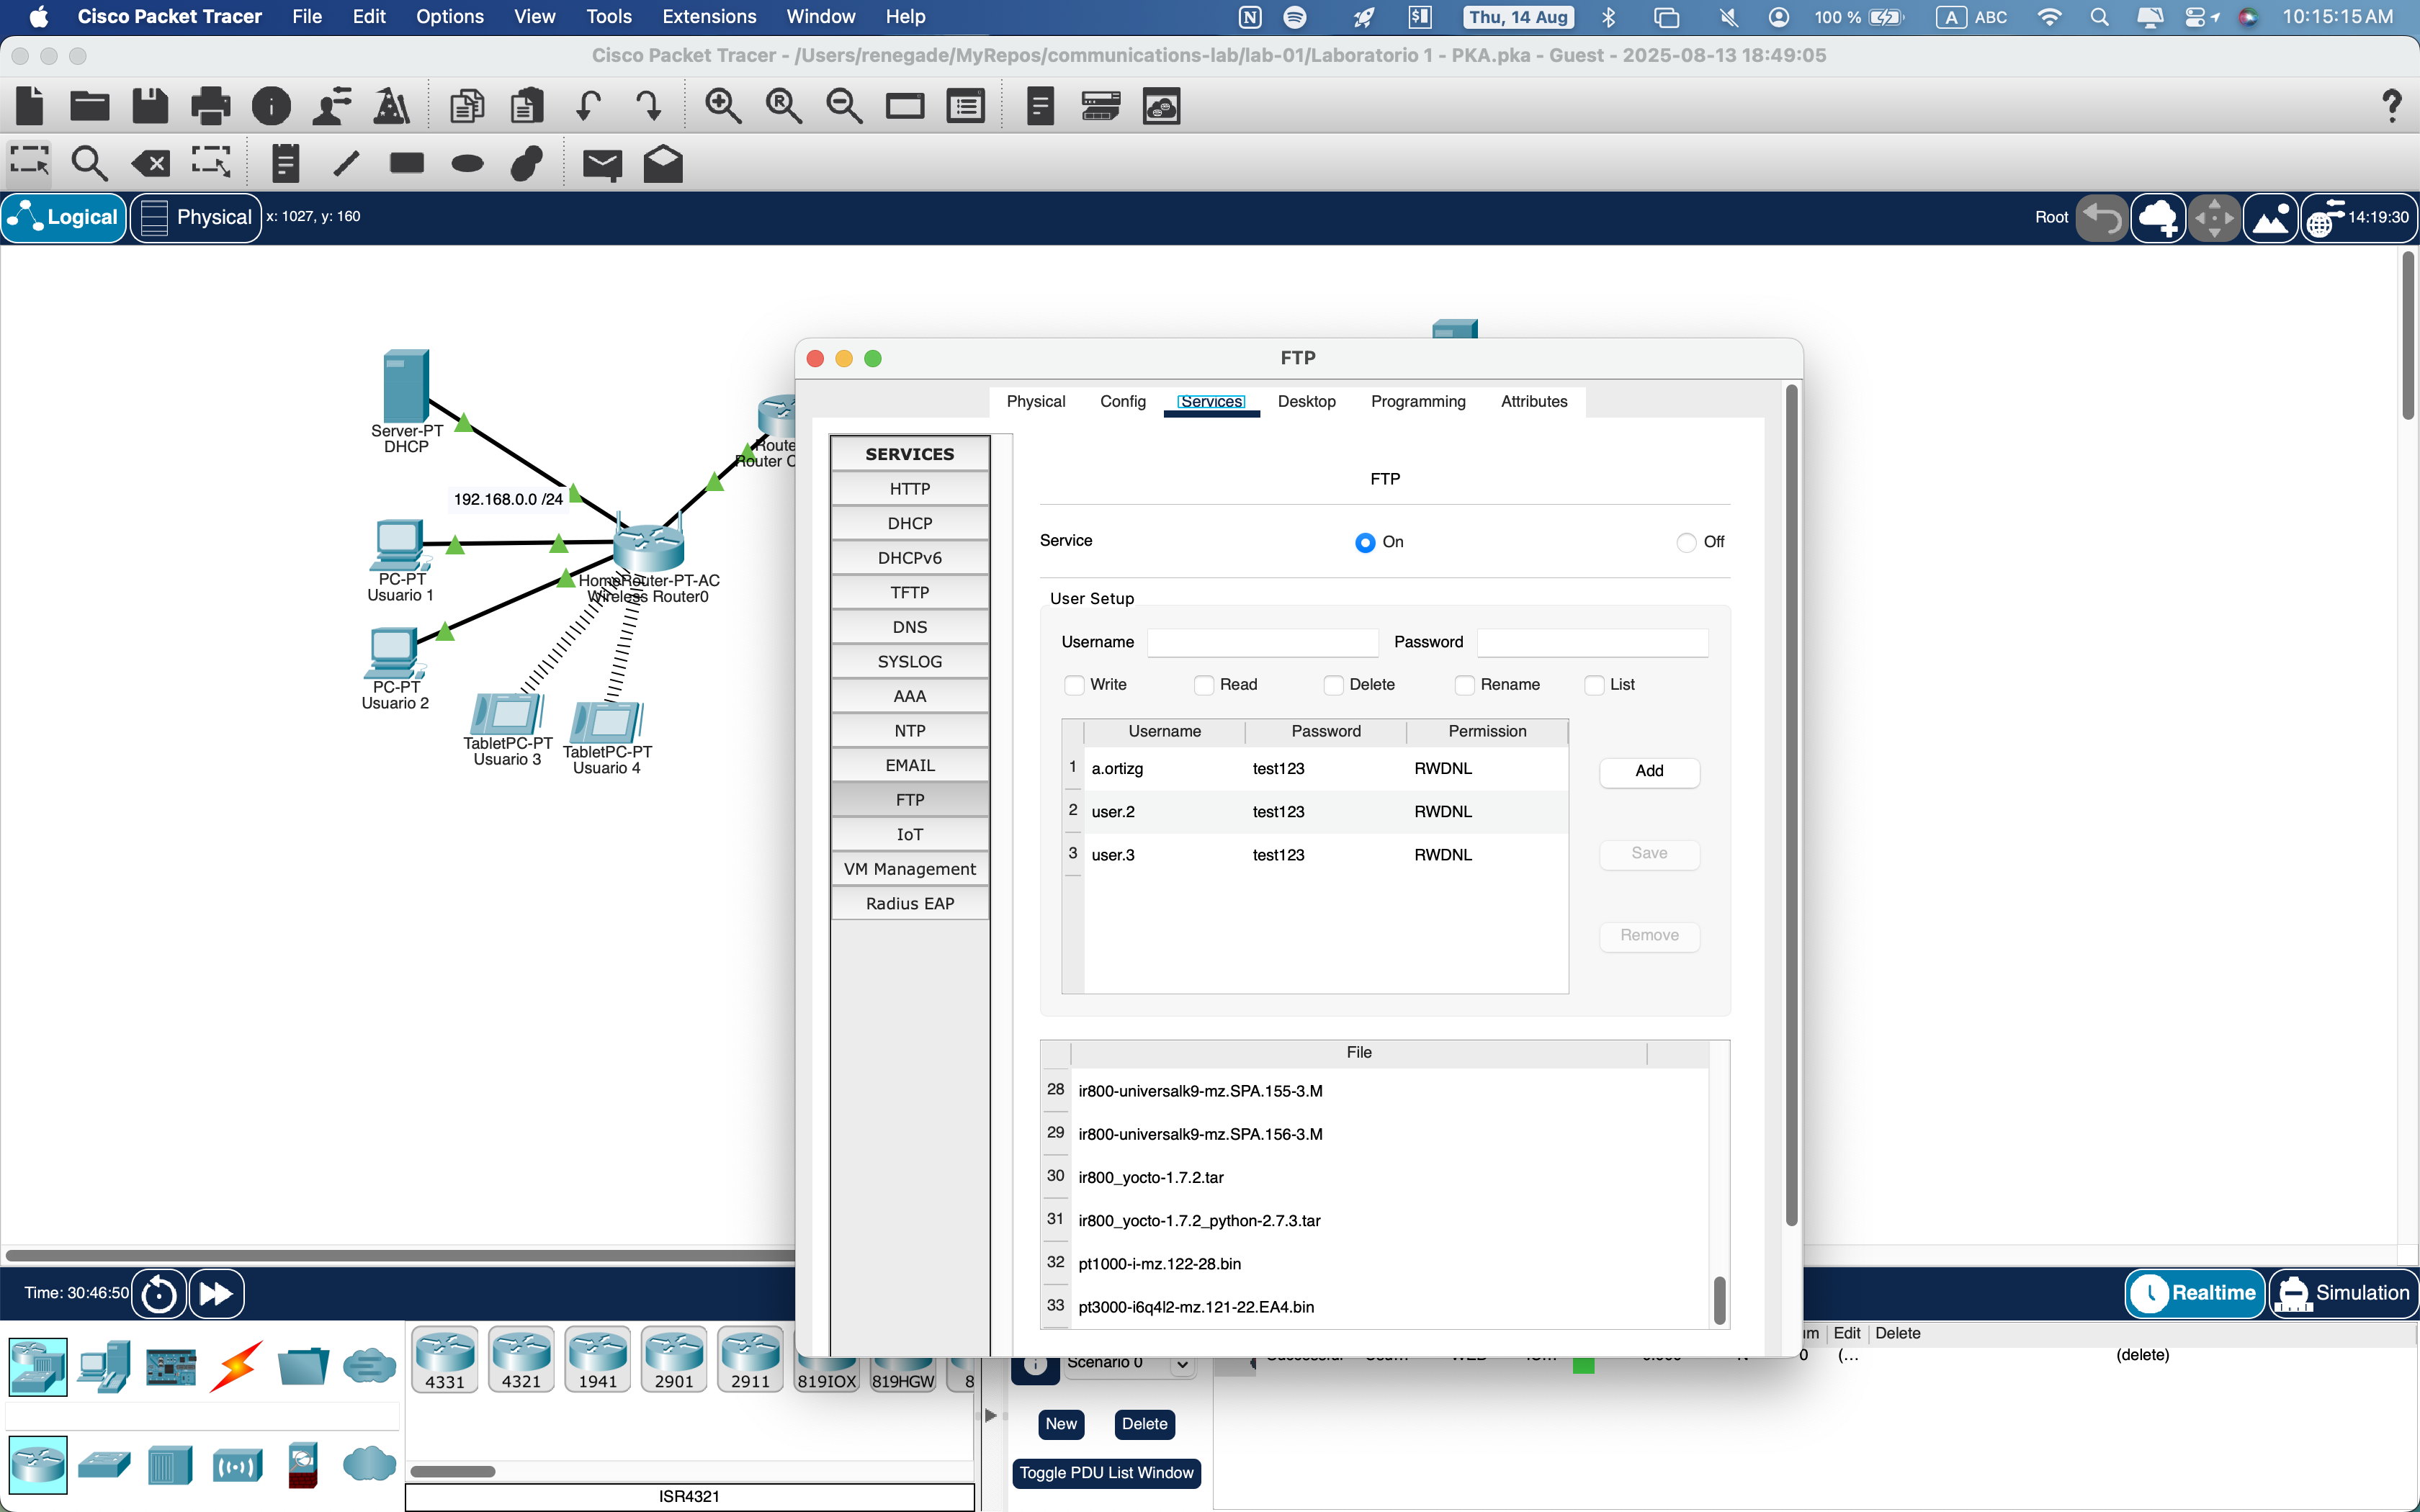
\includegraphics[width=0.65\textwidth]{lab-01-screenshots/46-1-ftp-config}
    \caption{Configuración de FTP server}
\end{figure}

\subsection{Configuración de usuarios en el FTP server}

Para lograr el envió de archivos entre cliente y servidor en nuestra red simulada, configuramos el FTP server. FTP funciona con dos canales: El canal de control (port 21) donde el cliente manda comandos y el servidor responde y el canal de datos (port 20) donde el contenido del archivo se mueve. En la figura 9 se ven las credenciales de los usuarios del FTP server.


\subsection{Prueba de conectividad al FTP server}
De forma similar a la prueba de conectividad al email server, también realizamos las prueba para el FTP server. 

\begin{figure}[H]
    \centering
    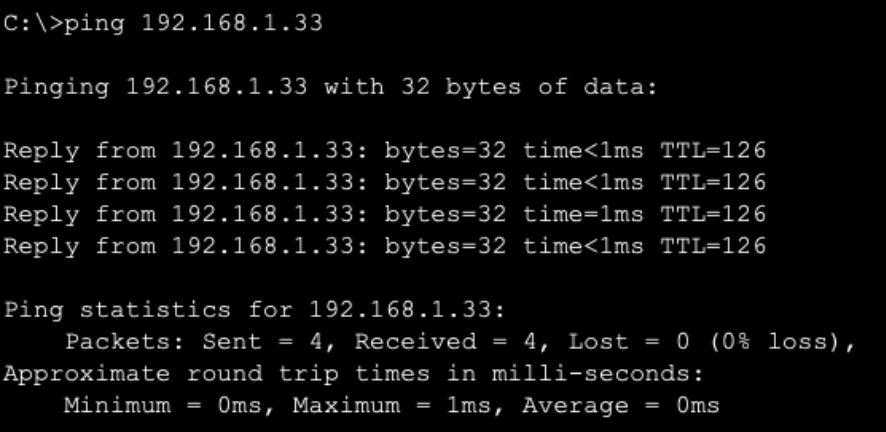
\includegraphics[width=0.65\textwidth]{lab-01-screenshots/46-2-ping-ftp}
    \caption{\textbf{ping} al FTP server}
\end{figure}

\subsection{Conexión y descarga de archvios al FTP server}
Para que un cliente configurado pueda descargar archivos del FTP server se conecta por medio del comando \textbf{ftp ftp.labredes.com}.El cliente luego corre \textbf{dir} y el servidor responde con la lista de archivos disponibles. El cliente luego realiza un GET paraindicarle al servidor que tiene que enviar el archvio. El servidor establece una   conexión separada para los datos en puerto 20 mientras que el canal de control permanece abierto. El servidor luego lee el archivo de almacenamiento y manda el contenido del archivo al cliente en un bit stream sobre el canal de datos. TCP se asegura de que el archivo llegue intacto. El cliente escribe los bits de llegada en un archivo locval nuevo y completa la descarga. Cuando se acaba la transferencia, el servidor cierra el canal de datos pero deja abierto el canal de control para recibir otro comando. 

\begin{figure}[H]
    \centering
    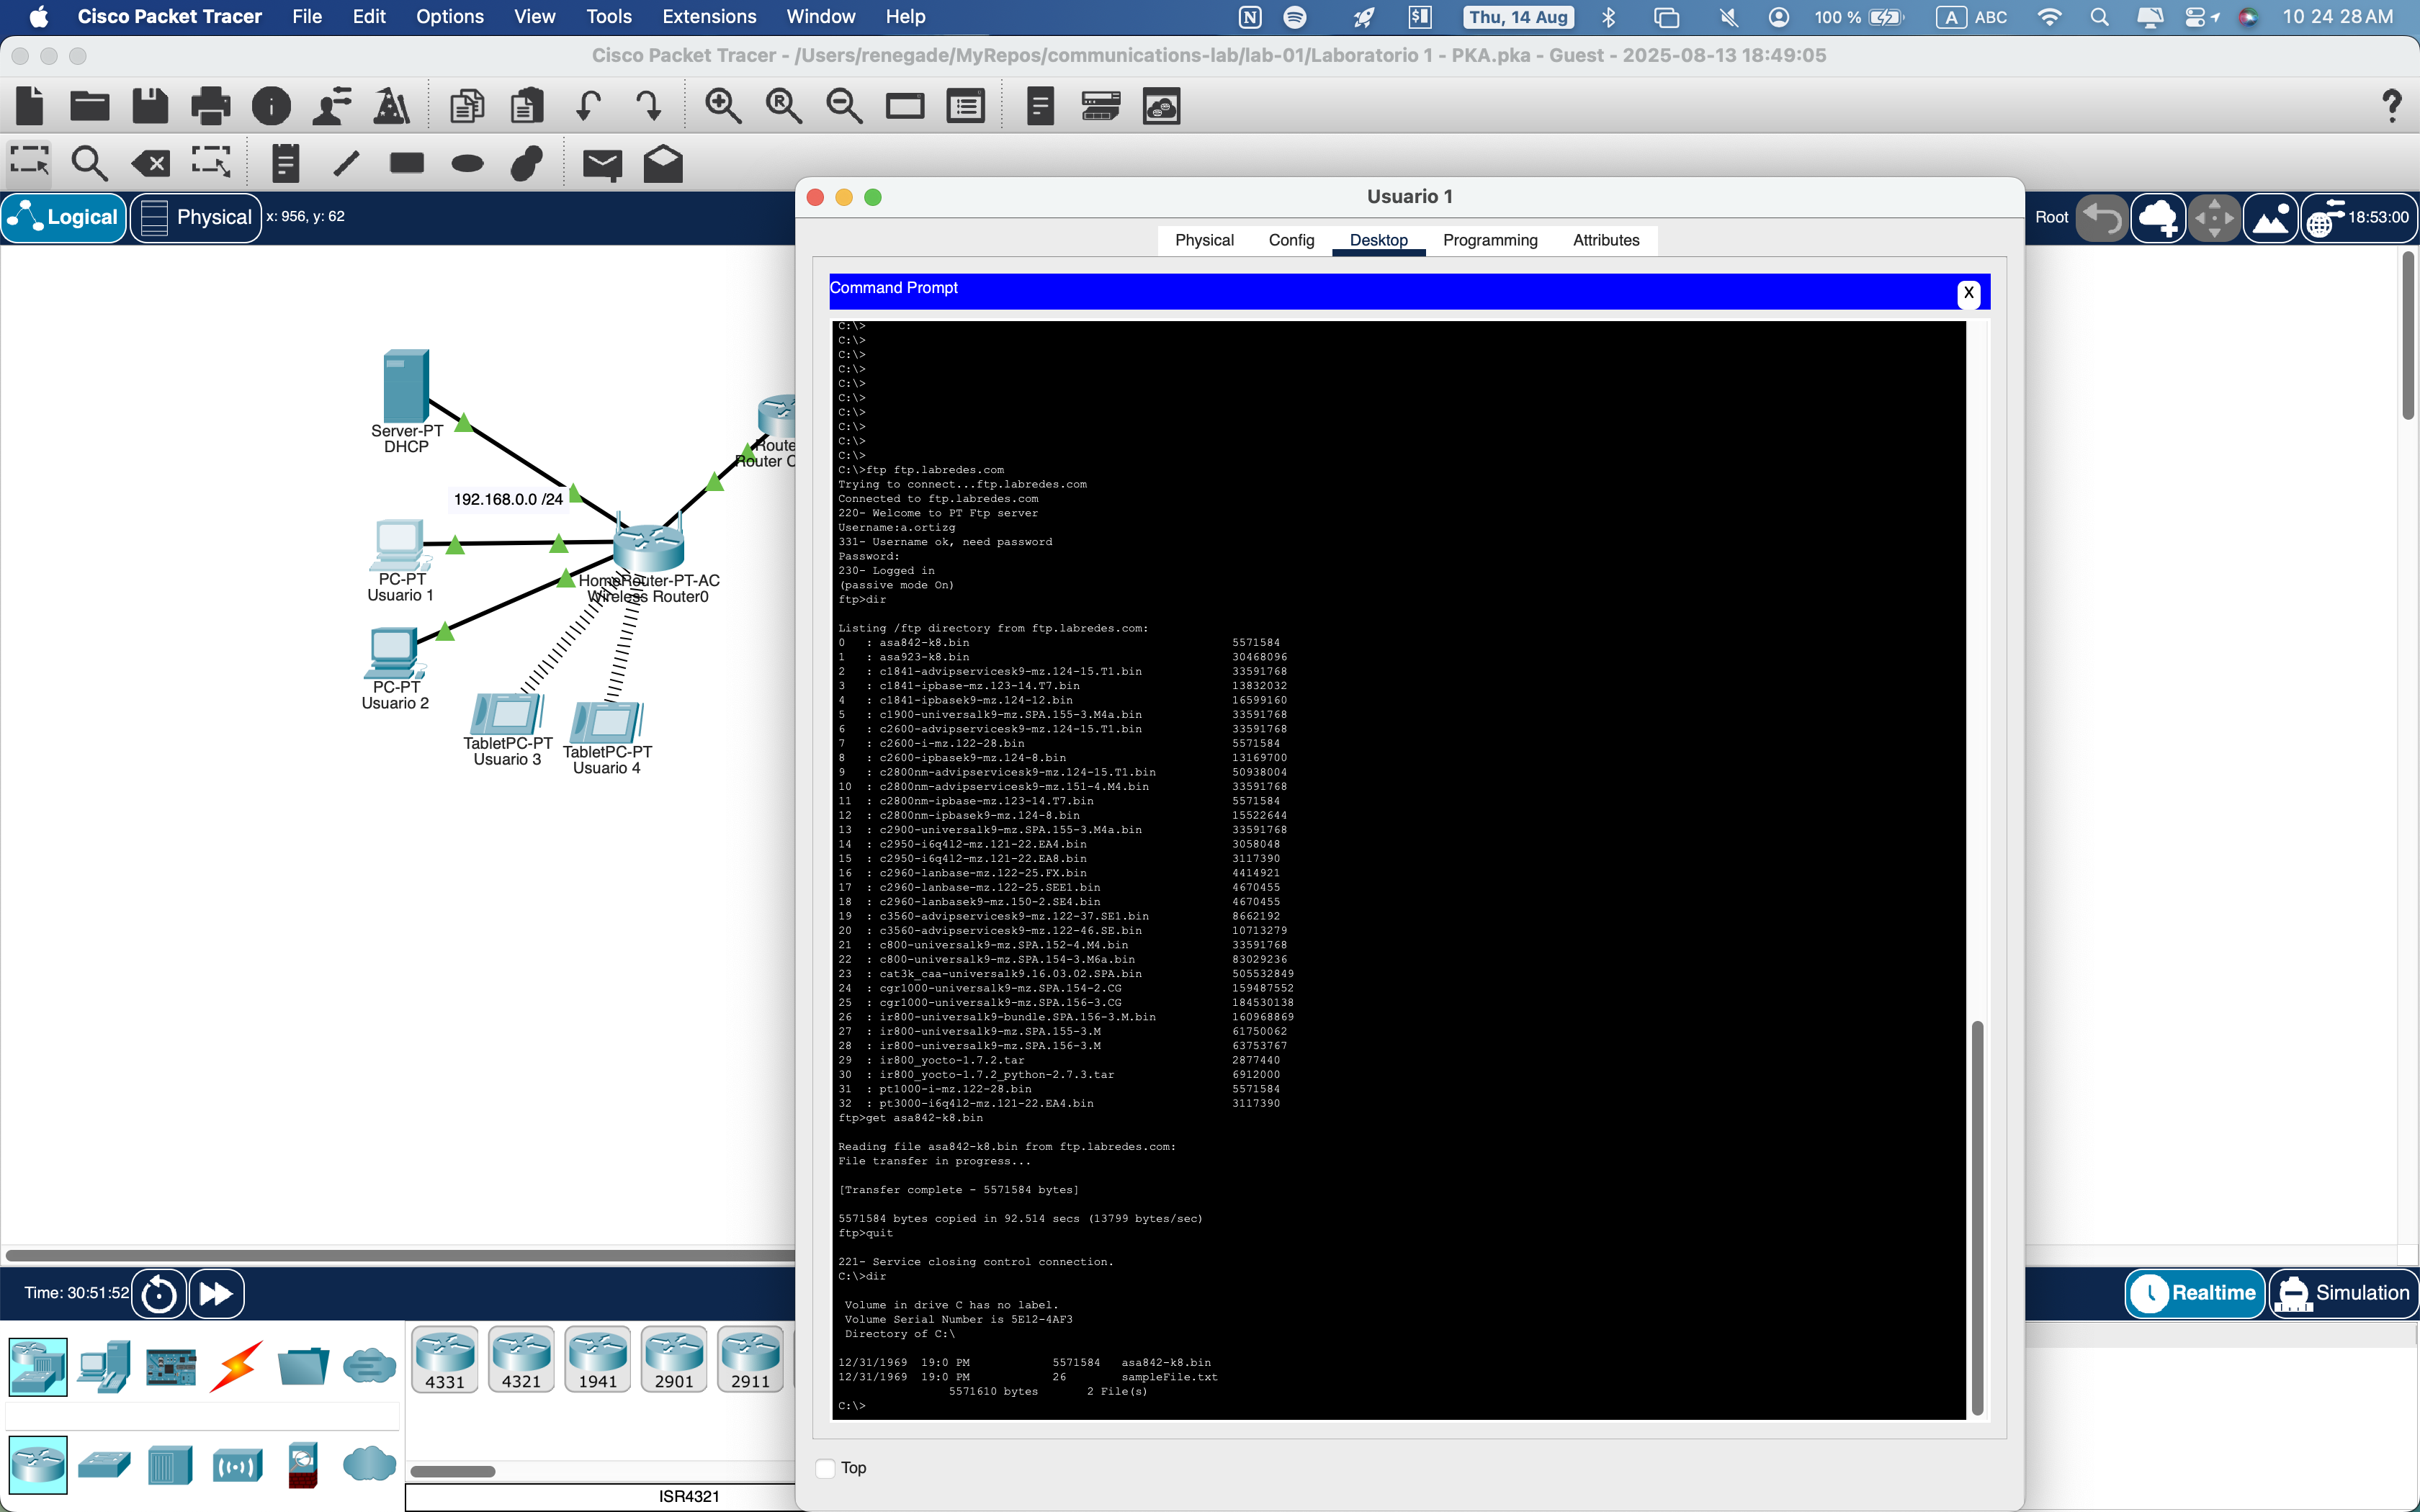
\includegraphics[width=0.65\textwidth]{lab-01-screenshots/46-3-get-ftp}
    \caption{Menu de FTP server y descarga de archivo}
\end{figure}

\begin{thebibliography}{9}

  \bibitem{cisco_tutorials}
  Cisco Packet Tracer Tutorials.

  \bibitem{cisco_ccna}
  Conceptos y Protocolos de Enrutamiento. Currícula Cisco CCNA Exploration.

  \bibitem{kurose_ross}
  Computer Networking, a top-down approach. James Kurose, Keith Ross. Addison-Wesley, 6th ed.

  \end{thebibliography}


\end{document}